\def\year{2019}\relax
%File: formatting-instruction.tex
\documentclass[letterpaper]{article} %DO NOT CHANGE THIS
%\newcommand{\CLASSINPUTbaselinestretch}{1.2}
%\documentclass[conference,twocolumn]{IEEEtran}
%\documentclass[letterpaper,10 pt,conference]{ieeeconf} 
%\documentclass[10pt, onecolumn]{IEEEtran}
%\documentclass[10pt,letterpaper]{article}
%\IEEEoverridecommandlockouts    
% \overrideIEEEmargins


%\usepackage[left=1in,top=1in,right=1in,bottom=1in]{geometry}


% \usepackage{geometry}
% \geometry{
% a4paper,
% total={210mm,297mm},
% left=17.1mm,
% right=17.1mm,
% top=19.1mm,
% bottom=17.1mm,
% }


\usepackage[english]{babel}
\usepackage{enumitem, hyperref}
\usepackage[latin1]{inputenc}
\usepackage{enumerate}
%\usepackage{enumitem}
%\setlist[enumerate]{label=\roman*}  %% for all enumerate environments
\usepackage{graphicx}
\usepackage{color}
\usepackage[dvipsnames]{xcolor}
\usepackage[T1]{fontenc}
\usepackage{subfigure}
%\usepackage{subcaption}
\usepackage{dsfont}
\usepackage{amsfonts}
\usepackage{graphicx,wrapfig}
\usepackage[T1]{fontenc}
\usepackage{amsmath}
\usepackage{mathtools, cuted}
\usepackage{amsthm}
\usepackage{amstext}
\usepackage{amssymb}
\usepackage{mathrsfs}
%\usepackage{cite}
\usepackage{mathtools}
\usepackage{tikz}
\usepackage{marginnote}
\usepackage{tkz-tab}
\usetikzlibrary{topaths,calc}
%*****Margin Note
\usepackage{stackengine}

%**********

\newcommand{\appsec}{
	\renewcommand{\thesubsection}{\Alph{subsection}}
}
\def\R{\mathbb{R}}
\def\cE{\mathcal{E}}
\def\fin{{<\infty}}
\def\supp{\mathop{\rm supp}}
\def\Gr{\mathop{\rm Gr}}
\def\cl{\mathop{\rm cl}}
\def\Proj{\mathop{\rm Proj}}
\def\argmax{\mathop{\rm arg\, max}}
\def\argmin{\mathop{\rm arg\, min}}
\def\eps{\varepsilon}
\def\hX{\hat{X}}
\def\hY{\hat{Y}}
\def\hx{\hat{x}}
\def\hf{\hat{f}}
\def\A{{\mathcal A}}
\def\B{{\mathcal B}}
\def\D{{\mathcal D}}
\def\F{{\mathcal F}}
\def\H{{\mathcal H}}
\def\I{{\mathcal I}}
\def\G{{\mathcal G}}
\def\C{{\mathcal C}}
\def\P{{\mathcal P}}
\def\Q{{\mathcal Q}}
\def\T{{\mathcal T}}
\def\X{{\mathcal X}}
\def\Y{{\mathcal Y}}
\def\M{{\mathcal M}}
\def\N{{\mathcal N}}
\def\S{{\mathcal S}}
\def\L{{\mathcal L}}
\def\cR{{\mathcal R}}
\def\Z{{\mathcal Z}}
\def\U{{\mathcal U}}
\def\V{{\mathcal V}}
%\newcommand{\indep}{\perp\!\!\!\perp}
\def\indep{{\perp\!\!\!\perp}}
\def\sgr{{\mathsf{gr}}}
\def\spr{{\mathsf{pr}}}
\def\sPr{{\mathsf{Pr}}}
\def\sUnif{{\mathsf{Unif}}}
\def\sBer{{\mathsf{Bernoulli}}}
\def\sP  {{\mathsf{P}}}
\def\sp{{\mathsf p}}
\def\sq{{\mathsf q}}
\def\sX{{\mathsf X}}
\def\sY{{\mathsf Y}}
\def\sZ{{\mathsf Z}}
\def\sM{{\mathsf {sENSR}}}
\def\sE{{\mathsf E}}
\def\sF{{\mathsf F}}
\def\sU{{\mathsf U}}
\def\sV{{\mathsf V}}
\def\sW{{\mathsf {W}}}
\def\sG{{\mathsf G}}
\def \var {{\mathsf {var}   }}
\def \mmse {{\mathsf {mmse}   }}
\def \cP {\mathsf{P}_{\mathsf{c}}}
\newcommand{\dsty}[1]{$\displaystyle #1$}
\def \AI {{I^{\mathsf{A}}}}
\def \nP {{\mathsf{P}^{(n)}}}
\def \np {{\mathsf{p}^{(n)}}}
\def \nq {{\mathsf{q}^{(n)}}}
\newcommand{\repdc}[3]{#1_{#2} , \ldots , #1_{#3}}
\usepackage[font=small,labelsep=space]{caption}
\captionsetup{%
	figurename=Fig.,
}
%\captionsetup{labelsep = }
\DeclareCaptionLabelSeparator{dot}{.~}
%\DeclareCaptionLabelSeparator{bar}{ | }
\captionsetup{
	labelsep=dot
}
%\theoremstyle{theorem}
%\theoremstyle{example}
\newcounter{example}
\newenvironment{example}[1][]{\refstepcounter{example}\par\medskip
	\noindent \textit{Example~\theexample. #1} \rmfamily}{\medskip}
%\newtheorem{example}{Example}
\newtheorem{definition}{Definition}
\newtheorem{theorem}{Theorem}
\newtheorem{corollary}{Corollary}
\newtheorem{fact}{Fact}
\newtheorem{proposition}{Proposition}
\newtheorem{lemma}{Lemma}
\theoremstyle{remark}
\newtheorem{remark}{Remark}
\newtheorem{conjecture}{Conjecture}
\newcommand{\markov}{\mathrel\multimap\joinrel\mathrel-%
	\mspace{-9mu}\joinrel\mathrel-}

\renewcommand{\qedsymbol}{\rule{0.5em}{0.5em}}
%%%%%%%%%%%%%%%%%%%%%%%%%%%%%%%%%%%%%%%%%%%%%%%%%%%%%%%%%%%%%%%%%%%%%%%%%%%%%%%%%%%%%%%%%55

\usepackage{times}
\usepackage{tikz}
\usepackage{amsmath}
\usepackage{verbatim}
\usetikzlibrary{arrows,shapes}
\tikzstyle{RectObject}=[rectangle,fill=white,draw,line width=0.2mm]
\tikzstyle{line}=[draw]
\tikzstyle{arrow}=[draw, -latex]
\usetikzlibrary{decorations.pathmorphing}
\usetikzlibrary{calc,shapes, positioning}
\usepackage{graphicx}
\usepackage{caption}
\usetikzlibrary{shapes.geometric}


\definecolor{DukeBlue}{HTML}{001A57}
\definecolor{DarkRed}{rgb}{0.75, 0.0, 0.0}
\definecolor{DarkGreen}{rgb}{0.0, 0.5, 0.0}
\newcommand{\TG}[1]{\textbf{\textcolor{DukeBlue}{(#1)}}}
\newcommand{\SK}[1]{\textbf{\textcolor{Magenta}{[#1]}}}
\newcommand{\md}[1]{\textcolor{Magenta}{#1}}



\DeclareFontFamily{U}{BOONDOX-calo}{\skewchar\font=45 }
\DeclareFontShape{U}{BOONDOX-calo}{m}{n}{
  <-> s*[1.05] BOONDOX-r-calo}{}
\DeclareFontShape{U}{BOONDOX-calo}{b}{n}{
  <-> s*[1.05] BOONDOX-b-calo}{}
\DeclareMathAlphabet{\mathcalboondox}{U}{BOONDOX-calo}{m}{n}
\SetMathAlphabet{\mathcalboondox}{bold}{U}{BOONDOX-calo}{b}{n}
\DeclareMathAlphabet{\mathbcalboondox}{U}{BOONDOX-calo}{b}{n}

%%%%%%%%%%%%%%%%%%%%%%%%%%%%%%%%%%%%%%%%%%%%%%%%%%%%%%%%%%%%%%%%%%%%%%%%%%%%%%%%%%%%%%%%5

% \IEEEoverridecommandlockouts

\allowdisplaybreaks

% Yi's delimiter
\newcommand{\paren}[1]{\left(#1\right)}
\newcommand{\set}[1]{\left\{#1\right\}}

\usepackage{aaai19}  %Required
\usepackage{times}  %Required
\usepackage{helvet}  %Required
\usepackage{courier}  %Required
\usepackage{url}  %Required
\usepackage{graphicx}  %Required
\frenchspacing  %Required
\setlength{\pdfpagewidth}{8.5in}  %Required
\setlength{\pdfpageheight}{11in}  %Required

%PDF Info Is Required:
\pdfinfo{
/Title (Wasserstein Soft Label Propagation on Hypergraphs: Algorithm and Generalization Error Bounds)
/Author (AAAI Press Staff)}
\setcounter{secnumdepth}{0}  

\begin{document}
% The file aaai.sty is the style file for AAAI Press 
% proceedings, working notes, and technical reports.
\title{Wasserstein Soft Label Propagation on Hypergraphs: Algorithm and Generalization Error Bounds}
\author{AAAI Press\\
Association for the Advancement of Artificial Intelligence\\
2275 East Bayshore Road, Suite 160\\
Palo Alto, California 94303\\
}
\maketitle

\begin{abstract}
Inspired by recent interests of developing machine learning and data mining algorithms on hypergraphs, we investigate in this paper the semi-supervised learning algorithm of propagating "soft labels" (e.g. probability distributions, class membership scores) over hypergraphs, by means of optimal transportation. Borrowing insights from Wasserstein propagation on graphs [Solomon et al. 2014], we re-formulate the label propagation procedure as message-passing algorithm, which renders itself naturally to a generalization applicable to hypergraphs through Wasserstein barycenters. Compared with Laplacian-based semi-supervised learning algorithms, the message-passing algorithm benefits from scalability and efficiency. Furthermore, in a PAC learning framework, we provide generalization error bounds for propagating one-dimensional distributions on graphs and hypergraphs using 2-Wasserstein distance, by establishing the \textit{algorithmic stability} of the proposed semi-supervised learning algorithm. These theoretical results also shed new lights upon deeper understandings of the Wasserstein propagation on graphs. 
%We validate the efficacy of the proposed algorithm through a number of synthetic and real data experiments.
\end{abstract}
	
\section{Introduction}
Recent decades have witnessed a growing interest in developing machine learning and data mining algorithms on \emph{hypergraphs} \cite{Hypergraph_Clustering,Hypergraph_Jost,Hypergraph_Game,Hypergraph_Kannan,Hypergraph_Olgica,Hypergraph_TV,HypergraphScalable}. As a natural generalization of graphs, a hypergraph is a combinatorial structure consists of vertices and hyperedges, where each hyperedge is allowed to connect any number of vertices. This additional flexibility facilitates capturing higher order interactions among objects; applications have been found in many fields such as computer vision \cite{Govindu2005}, network clustering \cite{Hyper_Spatial}, folksonomies \cite{GZCN2009}, cellular networks \cite{KHT2009}, and community detection \cite{KBG2018}.

This paper develops a probably approximately correct (PAC) learning framework for \emph{soft label propagation} or \emph{Wasserstein propagation} \cite{Solomon:2014}, a recently proposed semi-supervised learning algorithm based on optimal transport \cite{villani2003topics,villani2008optimal}, on graphs and hypergraphs. Different from the prototypical semi-supervised learning algorithm of \emph{label propagation} \cite{Belkin2004}, in which labels of interest are typically numerical or categorical variables, Wasserstein propagation aims at inferring unknown \emph{soft labels}, such as histograms or probability distributions, from known ones, based on pairwise similarities qualitatively characterized by edge connectivity and quantitatively measured using Wasserstein distances. Compared with traditional ``hard labels,'' soft labels are built with extra flexibility and informativeness, rendering themselves naturally to applications where uncertainty or distributional information is crucial. For instance, the traffic density at routers in the Internet network or topic distributions in the co-authorship network are more naturally modeled as probability distributions.

Briefly speaking, semi-supervised learning is a paradigm that leverages unlabelled data to improve the generalization performance for supervised learning, under generic, unsupervised structural assumptions (e.g. the manifold assumption) on the dataset; see \cite{Seeger01learningwith,Zhu06SSL,CSZ2006} for an overview. Given a graph $G=\left( V,E \right)$ and a subset of vertices $V_0\subset V$, label propagation is the procedure of extending an assignment of labels on $V_0$, denoted as a map $f_0:V_0\rightarrow \D$ valued in an arbitrary set $\D$, to a map $f:V\rightarrow\D$ on the entire vertex set $V$. Borrowing an analogy with classical heat equations, this extension procedure is reminiscent of heat propagation from ``boundary'' $V_0$ to the ``entire domain'' $V$. For soft label propagation, the label set $\D$ is the probability distributions $\P \left( N \right)$ modeled on a complete separable metric space $\left( N,d_N \right)$. %(which can be finite or countably/uncountably infinite), and the labeling maps are thus measure-valued.

Among the first works addressing semi-supervised learning with soft labels are \cite{Distribution_Propagation1,Distribution_Propagation2,SSL_Measure_Propagation}. In all these works, the similarity between two soft labels is quantitatively measured using the Kullback-Leibler (KL) divergence, which often suffers from instability and discontinuity for the inferred soft labels. In \cite{Solomon:2014} the authors proposed to replace the KL divergence with a $1$- or $2$-Wasserstein distance. The resulting soft label propagation algorithm is thus termed Wasserstein propagation. Specifically, given a measure-valued map $f_0:V_0\rightarrow\P \left( N \right)$ defined on $V_0\subset V$, Wasserstein propagation extends $f_0$ to $f:V\rightarrow \P \left( N \right)$ by solving the variational problem
\begin{equation}
  \label{eq:wasserstein-propagation}
  \min_{f:V\rightarrow\P \left( N \right)}\sum_{\left( v,w \right)\in E}W_p^p \left( f \left( v \right), f \left( w \right) \right)
\end{equation}
subject to the constraint $f\restriction V_0=f_0$. Here $W_p \left( \mu,\nu \right)$ denotes the $p$-Wasserstein distance between probability distributions $\mu,\nu\in\P \left( N \right)$ defined as
\begin{equation}
  \label{eq:wasserstein-distance}
  W_p \left( \mu,\nu \right)\coloneqq\inf_{\pi\in\Pi \left( \mu,\nu \right)}\left[\iint_{N\times N}d^p_N \left( x,y \right)\,\mathrm{d}\pi \left( x,y \right)\right]^{\frac{1}{p}}
\end{equation}
where $\Pi \left( \mu,\nu \right)$ is the set of all probabilistic couplings on $N\times N$ with $\mu$ and $\nu$ as marginals. When $p=2$, the minimizer of \eqref{eq:wasserstein-propagation} can be interpreted as a harmonic map, with boundary condition $f\restriction V_0=f_0$, that takes value in a weak, metric-measure space sense \cite{Otto2001,ambrosio2005gradient,LottVillani2009,Dirichlet_Wasserstein}. Note that this is a nontrivial fact because in general harmonic maps (or minimizers of the Dirichlet energy) only exist when the target metric space $\D$ is negatively curved in the sense of Alexandrov \cite{Jost}, but $\P \left( N \right)$ equipped with the $2$-Wasserstein distance has positive Alexandrov curvature \cite[\textsection 7.3]{ambrosio2005gradient}. When $\D$ is the one-dimensional distributions on the real line equipped with the $2$-Wasserstein distance, \cite{Solomon:2014} related \eqref{eq:wasserstein-propagation} to a Dirichlet problem.

In this work, we first extend the framework of \cite{Solomon:2014} to hypergraphs using \textit{Wasserstein barycenter} \cite{Wasserstein_Barycenter,Hypergraph_Asoodeh}. For $2$-Wasserstein distances this is equivalent to solving a \emph{multi-marginal optimal transport} \cite{CE2010} problem with a naturally constructed cost function. The hypergraph extension of Wasserstein propagation is based on a novel interpretation of the original algorithm on graphs \cite{Solomon:2014} as a message-passing algorithm. Next, we take a deeper look at the statistical learning aspects of our proposed algorithm, and establish generalization error bounds for propagating one-dimensional distributions on graphs and hypergraphs using the $2$-Wasserstein distance. One dimensional distributions such as histograms are among the most widely used applications. The main technical ingredient is \textit{algorithmic stability} \cite{Algorithmic_Stability}. To our knowledge, our generalization bound is the first of this type in the literature of Wasserstein distance based soft label propagation; on graphs these results generalize the generalization error bounds in \cite{Belkin2004}. As there is no general semi-supervised learning algorithm available for large dataset \cite{Label_Propa_100}, the new connection between Wasserstein barycenters and semi-supervised learning might be of theoretical as well as computational interest.  Due to the space constraint, \textit{some of the proof of the results presented in this paper are delegated to the Supplemental Material.}

%Our goal is to provide an efficient and theoretically sound approach to propagate probability measures $v\mapsto \mu_v$ on hypergraph $\H$ such that (i) $\mu_v$ coincide with the prescribed measures for $v\in V_0$ and (ii) all vertices within a hyperedge are assigned to "close" measures. To this goal, we reformulate Wasserstein label propagation \cite{Solomon:2014} as a message passing algorithm which renders  itself  naturally  to the hypergraph case via   We then provide generalization error bounds \cite{Generalization_semi} for propagating one-dimensional distributions on graphs and hypergraphs by establishing the 


%\subsection{Notation}
\noindent{\textbf{Notation.}} We denote an undirected simple graph $G$ as $G=(V, E)$ where $V=[n]\coloneqq\{1, \dots, n\}$ is the vertex set and $E\in V\times V$ denotes edges. We use $L$ to denote the (weighted) graph Laplacian associated with (weighted) graph $G$, which is a real square matrix of size $n$-by-$n$ defined by $L:=D-W$, where $W\in \mathbb{R}^{n\times n}$ is the (weighted) adjacency matrix of $G$, and $D\in \mathbb{R}^{n\times n}$ is a diagonal matrix with the (weighted) degree of vertex $j$ at its $\left( j,j \right)$-th entry. We use $H=(V, \mathcal E)$ to denote a hypergraph where $\mathcal E\in 2^V$ is the set of hyperedges of $H$. Given $k\geq 2$ probability measures $\rho_1, \dots, \rho_k$ in $\P(N)$, their \textit{Wasserstein barycenter} is %defined as %the minimizer of
\begin{equation}\label{Def:Barycenter}
    \mathsf{bar}\left(\{\rho_i\}_{i=1}^k\right)\coloneqq \inf_{\nu\in \P(N)}\frac{1}{k}\sum_{i=1}^nW_2^2(\rho_i, \nu).
\end{equation} 
Fundamental properties of the minimizer in \eqref{Def:Barycenter} are studied in \cite{Wasserstein_Barycenter}; similar results hold when the squared $2$-Wasserstein distance are weighted differently. Given a hyperedge $E$ of $H$, we use $\mathsf{bar}(E)$ to denote $\mathsf{bar}\left(\{\mu_i\}_{i=1}^{|E|}\right)$ where the probability measures $\mu_1, \dots, \mu_{|E|}$ associated with each vertex $i$ in 
$E$ are clear from the context.


\section{Message Passing and Label Propagation on Graph and Hypergraph}
In this section, we formulate our hypergraph label propagation as a special case of belief propagation. To this goal, we first briefly describe an slightly generalized version of Wasserstein label propagation \cite{Solomon:2014} from a message passing perspective.


A learning problem is specified by a probability distribution $D$ on $X\times Y$  according to which labeled sample pairs $z_i=\left( x_i,y_i \right)$ are drawn and presented to a learning algorithm. The soft label propagation problem amounts to setting $Y$ as a space of probability distributions and performs a regression problem for maps taking values in $Y$. Specifically, we let $Y$ be the simplex of probability distributions on a complete metric space $\left( N,d_N \right)$, i.e. $Y=\P\left( N \right)$. Since $N$ is complete, 
$Y$, equipped with Wasserstein distance, is a complete metric space \cite[Theorem 6.18]{villani2003topics}.
\subsection{Wasserstein Label Propagation for Graphs}
Let $X$ be a graph $G= \left( V,E \right)$, possibly with weights $\omega_{ij}$ on each edge $\left(i,j\right)$. Wasserstein label propagation is an extension of Tikhonov regularization framework on graphs \cite{Belkin2004} from real-valued functions to measure-valued maps. 
Denote a measure-valued map from $G$ to $\P\left( N \right)$ as $\mu:V\rightarrow\P\left( N \right)$. For simplicity, write $\mu_i:=\mu \left( i \right)$ for $i\in V$. A prototypical semi-supervised learning setting assumes $\mu_1,\cdots,\mu_m$ are known, where $1\leq m \ll n$, and the goal is to determine $\mu_{m+1},\cdots,\mu_n$ on the rest of the vertices. We will do so by minimizing the following objective function with Tikhonov regularization
\begin{equation}
  \label{eq:tikhonov}
  \min_{f:V\rightarrow \P\left( N \right)}\frac{1}{m}\sum_{i=1}^m W^2_2 \left( \mu_i,f_i \right)+\gamma\sum_{\left( i,j \right)\in E}\omega_{ij}W^2_2 \left( f_i,f_j \right),
\end{equation}
where $\gamma>0$ is a regularization parameter. This minimization problem can be thought of as an extension of the Dirichlet boundary problem studied in \cite{Solomon:2014} as here we do not impose $f_i=\mu_i$ for $i\in [m]$.
The minimizer of \eqref{eq:tikhonov} is the measure-valued map ``learned'' from the training data $\left\{ \left( i,\mu_i \right)\mid 1\leq i\leq n \right\}$ and the given graph structure $G= \left( V,E \right)$. We point out that the formulation in \cite{Solomon:2014} is a special case (parameter-free ``interpolated regularization'') of \eqref{eq:tikhonov} in the limit $\gamma\rightarrow0$, for the same reason as given in \cite[\textsection 2.2]{Belkin2004}.
%The presence of the knowledge about $G$ is what distinguishes semi-supervised learning from supervised learning: the vertices $m+1,\cdots,n$ can be thought of as ``unlabelled data'' made available to a semi-supervised learner.
 
%\begin{remark}
%  Though it is conceivable that the Tikhonov regularization framework can be potentially extended to other Wasserstein spaces $W_p$ with $0\leq p\neq 2$, we'll restrict our attention to $W_2$ since this is the Wasserstein space equipped with a natural Riemannian structure \cite{Otto2001,ambrosio2005gradient,LottVillani2009}.
%\end{remark}
% Let $L$ be the set of possible labels. For instance, for binary classification $L=\{0,1\}$ and for regression $L=\R$. "Soft" labels are therefore given by a probability distribution over $L$. We denote by $\P(L)$ the simplex of probability measures on $L$.
% Consider the minimization
% Consider the following minimization: 
% 	\begin{equation}
% 	  \label{Def:Minimization}
% 	  \min_{x\in \L^V}\sum_{C\in \C}f_C(x_C)
% 	\end{equation}
% where $V$ is the vertex set, $\C$ is the collection of subsets of $V$ and $f_C$ and $x_C$ correspond to functions and variables restricted to $C$.
% This minimization subsumes many unsupervised and semi-supervised learning settings. For instance, if we consider all neighboring pair of vertices, i.e. all $C$ with $|C|=2$ corresponding to $(i, j)\in E$, then we have
% 	\begin{equation}
% 	  \label{Def:Minimization2}
% 	  \min_{i\in \L^V}\sum_{i\in V}f_i(x_i) + \sum_{(i, j)\in E} f_{ij}(x_i, x_j)
% 	\end{equation}
% which is the classical formulation for SSL and/or metric labelling problem, see e.g., \cite{Image_Labeling}, where $f_i$ and $f_{ij}$ are called local \textit{unary} and 
% \textit{pairwise} energy terms. 
% The soft SSL approach in \cite{Solomon:2014} is also an special case of \eqref{Def:Minimization2} by choosing $x_i\in \P(L)$ for each $i\in V$, $f_i(x_i) = W(\mu_i, x_i)$ for $i\in V_0$ (the set of vertices with known labels) and $f_i(x_i)=0$ for $i\in V\backslash V_0$ and finally $f_{ij}(x_i, x_j) = W(x_i, x_j)$. 
We now provide an algorithm for solving \eqref{eq:tikhonov} based on belief propagation. Since this is only a motivating perspective, we assume for simplicity that the graph is unweighted; all arguments below can be extended to weighted graphs with heavier notations. In this context, each vertex $i$ updates its \textit{belief} about the local minimizer of \eqref{eq:tikhonov} $f_i$ by exchanging messages to edges it is incident to. The classical min-sum algorithm \cite{min_Sum} describes this process as follows. 
%Representing the graph $G=(V, E)$ as a \textit{factor graph}, we can cast the soft label propagation described in last section as a message passing. Each $v\in V$ is a \textit{variable node} and each $e\in E$ is a \textit{factor node}.	
%Denote the set of edges with direction distinguished by $\vec{E}=\{(i,j)\in V\times V:j\in N(i)\}$.
At time $t$, vertex $i\in [m]$ has belief $b^{(t)}_i$ about the minimizer $f_i$ of \eqref{eq:tikhonov}; then, at time $t+1$, $i$ sends message $J^{(t)}_{i\to e}$ to edge $e=(i, j)$ and receives message $J^{(t)}_{e\to i}$ from $e$, updating the message for next iteration according to
% there are two messages on each edge $(i, e)\in E'$ in two different direction: $i\in V$ sends a message $J^{(t)}_{i\to e}:R\to R$ to $e=(i, j)\in E$ and receives a message $J^{(t)}_{e\to i}:R\to R$ from $e$:
\begin{equation}\label{Eq:Update2}
J^{(t)}_{i\to e} \left(b^{(t)}_i\right) = W_2^2\left(\mu_i, b^{(t)}_i\right) + \sum_{k\in N(i)\backslash \{j\}}J^{(t-1)}_{(i,k)\to i}\left(b^{(t-1)}_i\right)
\end{equation}
and 
\begin{equation}\label{Eq:Update}
    J^{(t)}_{e\to i}\left(b^{(t)}_i\right) =  \min_{f_j\in \P(N)}\left[W_2^2\left(b^{(t)}_i, f_j\right) + J^{(t-1)}_{j\to e}\left(f_j\right)\right].
\end{equation}
The first term in \eqref{Eq:Update2} is set to be zero if $i\notin [m]$. The belief is then updated at at time $t+1$ according to evolution
\begin{equation*}
b^{(t+1)}_i \coloneqq \argmin_{f_i} \left[W_2(\mu_i, f_i) + \sum_{k\in V: (i, k)\in E } J^{(t)}_{(i, k)\to i}(f_i)\right].
\end{equation*}
Convergence of $b_i^{(t)}$ to the true minimizer $f^*_i$ can be guaranteed under some (mild) conditions on initial beliefs if $G$ is a tree (see e.g., \cite{min_Sum}).
% {\color{blue}Just remember that the idea of "factor graph" and bringing "factor nodes" in the simple graph case just makes everything messier! Because the above two equations can be easily combined as the following: 
% \begin{equation}\label{Eq:Update}
%     J^{(t)}_{j\to i}(x_i) =  \min_{x_j}\Big[f_i(x_j) + f_{ij}(x_i, x_j) + \sum_{v\in N(j)\backslash i}J^{(t-1)}_{v\to i}(x_j)\Big].
% \end{equation}
% }
% keeps track of a \textit{message} from each neighbor $u\in N(i)$ where this message is denoted as $J^{(t)}_{i\to i}:R\to R$. These incoming messages are combined to compute new outgoing messages for each neighbor. The message $J^{(t+1)}_{i\to j}(\cdot)$ from vertex $i$ to vertex $j\in N(i)$ evolves according to
% \begin{equation}\label{Eq:Update}
%     J^{(t+1)}_{i\to j}(x_j) =  \min_{y_i}\Big[f_i(y_i) + f_{ij}(y_i, x_j) + \sum_{v\in N(i)\backslash j}J^{(t)}_{v\to i}(y_i)\Big].
% \end{equation}
%At each time $t$, the \textit{belief} of local minimizer $x^*_i$ is defined as 
%$$b^{(t)}_i(x_i) = f_i(x_i) + \sum_{e\in E: (i, e)\in E'} J^{(t)}_{e\to i}(x_i).$$ 
% If the true global minimizer $f^*$ is unique (for instance under the strict convexity assumption), then $|\argmin_{x_i} b_i^{(t)}(x_i)|=1$ for all $i$ and sufficiently large $t$. Therefore, we define an estimate of the minimizer $x^{(t)}_i$ for vertex node $i$ is then given by 
% $$x_i^{(t)} = \argmin_{y_i} b^{(t)}_i(x_i).$$

%$$x_i^{(t)} = \argmin_{y_i}f_i(y_i) +\sum_{v\in N(i)}J^{(t)}_{v\to i}(y_i).$$ 

\subsection{Wasserstein Label Propagation for Hypergraph}
Let now $X$ be represented by a hypergraph $H=(V, \mathcal E)$. Since each hyperedge may contain arbitrary number of vertices, the minimization \eqref{eq:tikhonov} fails to formulate our learning objective. Nevertheless, the belief propagation updates \eqref{Eq:Update2} and \eqref{Eq:Update} can naturally be extended to the message passing between vertex $i$ and hyperedge $E$ containing $i$ as 
\begin{equation}\label{Eq:Update_H_2}
J^{(t)}_{i\to E} \left(b_i^{(t)}\right) = W_2^2\left(\mu_i, b_i^{(t)}\right) + \sum_{E'\in \mathcal E\backslash\{E\}: i\in E'}J^{(t-1)}_{E'\to i}\left(b_i^{(t-1)}\right)
\end{equation}
and 
\begin{equation}\label{Eq:Update_H}
    J^{(t)}_{E\to i}\left(b_i^{(t)}\right) =  \min_{f_{E\backslash \{i\}}}\Big[\mathsf{bar}(E) + \sum_{k\in E\backslash \{i\}}J^{(t-1)}_{k\to E}(f_k)\Big].
\end{equation}
where  $f_{E\backslash \{i\}}=\{f_k\in\P(N): k\in E\backslash\{i\}\}$.
% We construct the factor graph $(V\cup \mathcal E, E')$ corresponding to $H$. Unlike the simple graph case, each factor node (i.e., hyperedge) $E$ has degree larger than 2. The messages over factor graph evolve as the following:

% $$J^{(t)}_{i\to E} (x_i) = f_i(x_i) + \sum_{\hat E\in \mathcal E\backslash\{E\}: i\in \hat E}J^{(t-1)}_{\hat E\to i}(x_i)$$
% and 
% \begin{equation}\label{Eq:Update}
%     J^{(t)}_{E\to i}(x_i) =  \min_{x_{E\backslash \{i\}}}\Big[\mathsf{bar}(E) + \sum_{k\in E\backslash \{i\}}J^{(t-1)}_{k\to E}(x_k)\Big].
% \end{equation}
% In above, we use $x_{E\backslash \{i\}}$ to denote the set of probability measures corresponding to vertices in $E$ expect for vertex $i$ whose probability measure is fixed $x_i$.
The belief of vertex $i\in [m]$ is then obtained according to the following rule:
$$b_i^{(t+1)}=\argmin_{f_i\in \P(N)}\left[W_2^2(\mu_i, f_i) + \sum_{E\in \mathcal{E}:i\in E}J^{(t)}_{E\to i}(f_i)\right].$$


This belief propagation update rules justify the following formulation of label propagation for hypergraphs
\begin{equation}\label{eq:tikhonoc_Hyper}
    \min_{f:V\to \P(N)} \frac{1}{m}\sum_{i=1}^m W_2^2\left(\mu_i, f_i\right) + \gamma\sum_{E\in \mathcal E}\mathsf{bar}(E)
\end{equation}
which is a natural generalization of \eqref{eq:tikhonov} when the graph is unweighted. For weighted graphs, \eqref{eq:tikhonoc_Hyper} still holds with properly adjusted $\mathsf{bar}(E)$ with weights.

\section{Propagating One-Dimensional Distributions with $2$-Wasserstein Distances}
In this section, we assume that the labels are one-dimensional probability distributions, i.e., $N\subset \R$, and work solely with the $2$-Wasserstein distance. We will see that in this case hypergraph label propagation can be cast into a Wasserstein propagation on a weighted graph arising from the clique representation of the hypergraph. Therefore, in the rest of this paper it suffices to establish generalization error bounds for standard graphs.

Given a hypergraph $H=(V, \mathcal E)$, we define its \textit{clique representation} as a graph $G_H=(V, E_H)$, where $E_H=\{(i, j):\exists E\in \mathcal E, \{i, j\}\subset E\}$. The main advantage of one-dimensional soft labels is illustrated by the following classical result in optimal transportation theory.
\begin{theorem}[\cite{villani2003topics}]\label{Thm:Wasserstein_One}
Let $\mu, \nu\in \P(N)$ with $N\subset\R$ with cumulative density functions (c.d.f.) $F_\mu$ and $F_\nu$, respectively. Then $$W_2^2(\mu, \nu)=\int_{0}^1\left(F_\mu^{-1}(s)-F_\nu^{-1}(s)\right)^2\text{d}s,$$
where $F_{\mu}^{-1}$ and $F_{\nu}^{-1}$ are the generalized inverses of $F_\mu$ and $F_\nu$, respectively, i.e., $F_\mu^{-1}(s)\coloneqq \inf\{x\in N:F_\mu(x)>s\}$. 
\end{theorem}
The explicit expression for Wasserstein distance enables us to derive the barycenter of any number of one-dimensional distributions in a closed form. 
\begin{theorem}[\cite{bigot2017}]
\label{Thm:Barycenter_One}
Let $\rho_1, \dots, \rho_k\in \P(N)$ be $m$ probability distributions on $N\subset\R$ with cumulative density functions $F_{\rho_i}$, $i\in [k]$. Let $\rho_{\mathsf{b}}$ be the (unique) Wasserstein barycenter of $\{\rho_i\}_{i=1}^k$. Then the generalized inverse c.d.f.\ $F^{-1}_{\mathsf{b}}$ of $\rho_{\mathsf{b}}$ is given by 
$$F^{-1}_{\mathsf{b}}(s)=\frac{1}{k}\sum_{i=1}^kF_{\rho_i}^{-1}(s).$$
\end{theorem}
Since the inverse cdf's and the distributions are in one-to-one correspondence, this theorem characterizes the $2$-Wasserstein barycenter of $\{\rho_i\}_{i=1}^m$. In light of Theorem~\ref{Thm:Barycenter_One}, one can simplify the barycenter of hyperedge $E$ that contains vertices, say, $\{1, 2, \dots, k\}$ as
\begin{eqnarray}
\mathsf{bar}(E) &=& \frac{1}{k}\sum_{i=1}^kW^2_2(\mu_i, \mu_\mathsf{b})\nonumber\\
%&=&\frac{1}{k}\sum_{i=1}^k\int_{0}^1\left(F_{\mu_i}^{-1}(s)-F_\mathsf{b}^{-1}(s)\right)^2\text{d}s\nonumber\\
&=&\frac{1}{k}\sum_{i=1}^k\int_{0}^{1}\left(F_{\mu_i}^{-1}(s)-\frac{1}{k}\sum_{i=1}^kF_{\mu_i}^{-1}(s)\right)^2\text{d}s\nonumber\\
&=&\frac{1}{k^2}\sum_{i=1}^k\sum_{j=i+1}^n\int_0^1\left(F_{\mu_i}^{-1}(s)-F_{\mu_j}^{-1}(s)\right)^2 \text{d}s \nonumber\\
&=&\frac{1}{k^2}\sum_{i=1}^k\sum_{j=i+1}^kW_2^2(\mu_i, \mu_j)\label{Eq:One_D_Equivalence}
\end{eqnarray}
where the first and second equalities follow from Theorems~\ref{Thm:Wasserstein_One} and \ref{Thm:Barycenter_One}, respectively. Comparing \eqref{Eq:One_D_Equivalence} with \eqref{eq:tikhonoc_Hyper}, we have
\begin{proposition}
  \label{prop:clique-equivalence}
  Soft label propagation with $2$-Wasserstein distance for one-dimensional distributions on hypergraphs $H$ using \eqref{eq:tikhonoc_Hyper} is equivalent to Wasserstein propagation on a weighted graph arising from the clique representation $G_H$ of $H$. The weight of each edge $e$ in $G_H$ depends only on the degrees of the hyperedges containing $e$.
\end{proposition}

%It follows from \eqref{Eq:One_D_Equivalence} that in one-dimensional case the $2$-Wasserstein barycenter of each hyperedge of $H$ is given by the weighted average Wasserstein distance of the corresponding clique representation $G_H$. In particular,  %Consequently, label propagation for hypergraph formulated in \eqref{eq:tikhonoc_Hyper} is equivalent to Wasserstein label propagation for graph given in  \eqref{eq:tikhonov}. This then motivates us to concentrate on the latter as the label propagation for both graph and hypergraph.

\section{Generalization Bounds for Wasserstein Label Propagation}
In this section, we focus on label propagation \eqref{eq:tikhonov} (for both graph and hypergraph) and derive generalization bounds. Before proceeding, we briefly review empirical risk, generalization error, and algorithmic stability in the passing.
% \subsection{Generalization error}
% In the \emph{Probably Approximately Correct} (PAC) framework, we assume the truth $\left\{ \left( i,\mu_i \right)\mid 1\leq i\leq n \right\}$ is sampled i.i.d.\ from a joint distribution $\theta\in \P\left( V\times \P\left( N \right) \right)$. We denote the \emph{empirical risk} or \emph{empirical error} by
% \begin{equation}
%   \label{eq:empirical-risk}
%   R_m \left( f \right)=\frac{1}{m}\sum_{i=1}^mW_2 \left( \mu_i, f_i \right)
% \end{equation}
% and the \emph{generalization error} by
% \begin{equation}
%   \label{eq:generalization-error}
%   R_{\theta} \left( f \right)=\mathbb{E}_{\theta} W_2 \left( f_i, \mu_i \right)
% \end{equation}
% where the expectation is taken over the joint distribution $\theta$.
% One subtlety in these theoretical assumption is whether one should allow the vertices $V=\left[ n \right]$ to be sampled with replacement. In fact, in order for the training samples to be i.i.d.\ drawn from a joint distribution on $V\times \P\left( N \right)$, it is inevitably to allow for multiplicity. Intuitively, one could expect that the probability of drawing repeated vertices in the graph should not be large if $m\ll n$, provided that the marginal distribution of $\theta$ on $G$ is "sufficiently close to uniform." Therefore, it should suffice if we impose an additional assumption for upper bounding the maximum multiplicity of the vertices sampled, since any generalization error bound we establish subsequently will be probabilistic anyways. {\color{blue} Keep this?}

% To be able to talk about i.i.d.\ samples in a sensible way, we allow for multiplicities of graph vertices in the training sample $S=\left\{ \left( v_i,\mu_i \right)\mid 1\leq i\leq m,\,\,v_i\in V,\,\,\mu_i\in\P\left( N \right) \right\}$, where each $v_i\in V$ is an integer between $1$ and $n=\left| V \right|$. In principle it may well be possible that $m>n$, but we assume the number of distinct elements among $v_1,\cdots,v_m$ is strictly less than $n$. Denote the number of distinct elements among $v_1,\cdots,v_m$ by $\ell$, where $1\leq \ell<n$. While it still makes sense if $\ell=n$, in this case the learning problem could be better addressed as a denoising problem. For notational simplicity, we assume without loss of generality that the distinct vertices among $v_1,\cdots,v_m$ are the first $\ell$ vertices in the graph, and vertex $i\in V$ appears in $S$ with multiplicity $t_i\geq 1$.


\subsection{Algorithmic Stability}  
The framework of algorithmic stability \cite{DW1979,Algorithmic_Stability,MNPR2006} was proposed in statistical learning as an alternative to the VC-dimension framework; the latter is often over-pessimistic since it attempts to bound the generalization performance uniformly over all algorithm. We briefly recapture the essence of algorithmic stability here. Let $X$ and $Y$ be two measurable spaces, and a set of training samples $S=\left\{ z_1=\left( x_1,y_1 \right),\cdots,z_m= \left( x_m, y_m \right) \right\}$ of size $m$ sampled i.i.d. with respect to an unknown joint distribution $D$ on the product space $Z=X\times Y$. A learning algorithm is a mechanism that maps $S$ to a global map $f_S:X\rightarrow Y$ defined on the entire $X$. It is often assumed for simplicity that the algorithm is symmetric with respect to training sets, i.e., the learning algorithm should return identical maps for two training sets with samples differing from each other only by a permutation. We shall assume all maps considered here are measurable, and all the measure spaces are separable. In the scenario of main interest to us in this paper, $X$ is the simple finite graph and $Y$ is the probability space $\P\left( N \right)$. The \emph{empirical risk} or \emph{empirical error} of a mapping $f_S:X\rightarrow Y$ learned from the training set $S$ of size $m>0$ is defined as
\begin{equation*}
  R_m \left( f_S \right):=\frac{1}{m}\sum_{i=1}^mc \left( f_S, z_i \right)
\end{equation*}
where $c \left( \cdot,\cdot \right):Y^X\times \left( X\times Y \right)\rightarrow\mathbb{R}_{\geq0}$ is a cost function evaluating the predictive error of $f_S:X\rightarrow Y$ at a point sampled from the joint distribution $D$ on $X\times Y$. The \emph{generalization error} of the learned map $f_S:X\times Y$ is
\begin{equation*}
  R_D \left( f_S \right)=\mathbb{E}_{z\sim D} \left[ c \left( f_S,z \right) \right].
\end{equation*}
Intuitively, the generalization error measures the average prediction error for a map learned from  training data. The PAC learning framework is centered at bounding the discrepancy between $R_m$ and $R_D$. In \cite{Algorithmic_Stability}, the authors proved that such a bound can be obtained if the algorithm satisfies a \emph{uniform stability} property. 

\begin{definition}[Uniform Stability, \cite{Algorithmic_Stability}]
  \label{defn:uniform-stability}
  Fix a positive integer $m\in\mathbb{Z}_+$. Let $S=\left\{ z_1,\cdots,z_m \right\}\subset X\times Y$ be a training set, and $S'$ be another training set that contains the same elements as $S$ with the only exception that the sample $z_i$ is replaced with a different sample $z_i'\neq z_i$. A learning algorithm $A:\left( X\times Y \right)^m\rightarrow Y^X$ that sends any training set $S$ to a mapping $f_S:X\times Y$ is said to be (uniform) $\beta$-stable for some positive constant $\beta>0$ if for any pair of training sets $S$, $S'$ differing by exact one element the following inequality holds:
  \begin{equation*}
    \left| c \left( f_S,z \right)-c\left(f_{S'},z\right) \right|\leq \beta\qquad\forall z\in X\times Y.
  \end{equation*}
\end{definition}
Note that uniform stability is a very strong property: if the training sample undergoes a small change, the learned mapping will also change very little in terms of predictive power. Of course the order of $\beta$ in terms of the number $m$ of training samples will be crucial here, otherwise any learning algorithm is uniformly stable for any bounded cost function.

\begin{theorem}[\cite{Algorithmic_Stability}]
  \label{thm:bousquet-elisseeff}
  Let $S\mapsto f_S$ be a $\beta$-stable learning algorithm, such that $0\leq c \left( f_S,z \right)\leq M$ for all $z\in X\times Y$ and all learning set $S$. For any arbitrary $\epsilon>0$ we have for all $m\geq 8M^2/\epsilon^2$
  \begin{equation}
    \label{eq:fraction-bounds}
    \begin{aligned}
    \mathbb{P}_{S\sim D^m} &\left\{ \left| R_m \left( f_S \right)-R_D \left( f_S \right) \right| > \epsilon\right\}\leq \frac{64 Mm\beta+8M^2}{m\epsilon^2},
    \end{aligned}
  \end{equation}
  and for any $m\geq 1$
  \begin{equation}
    \label{eq:exponential-bounds}
    \begin{aligned}
    \mathbb{P}_{S\sim D^m}&\left\{ \left| R_m \left( f_S \right)-R_D \left( f_S \right) \right| > \epsilon+\beta\right\}\\
    &\qquad\qquad\leq 2\exp \left( -\frac{m\epsilon^2}{2 \left( m\beta+M \right)^2} \right).
    \end{aligned}
  \end{equation}
\end{theorem}
As pointed out in \cite{Algorithmic_Stability}, in order for these bounds to be tight, a sufficient condition is that $\beta$ grows like $O \left( 1/m \right)$ as $m\rightarrow\infty$. It was verified in \cite{Algorithmic_Stability} that the Tikhonov regularization framework with quadratic cost function satisfies this requirement. Theorem~\ref{thm:bousquet-elisseeff} is very general---it is applicable to any measurable spaces $X$ and $Y$. The rest of this paper is devoted to establishing algorithmic stability for the (hyper)graph soft label propagation algorithms. %satisfies this framework, we should be able to conclude that generalization bounds \eqref{eq:fraction-bounds} and \eqref{eq:exponential-bounds} hold for the soft label propagation on graphs.

\subsection{Generalization bounds for Soft Label Propagation} 
The goal of this subsection is to verify that the conditions of Theorem~\ref{thm:bousquet-elisseeff} are satisfied for the Tikhonov regularization framework \eqref{eq:tikhonov}.
The first task is to find an appropriate model class for the distributions in $\P\left( N \right)$ that ensures the uniform boundedness of the cost function
\begin{equation}
  \label{eq:wasserstein-cost-func}
    c\left( f, \left( j,\mu_j \right) \right)=W_2^2 \left( f_j,\mu_j \right).
\end{equation}
This can be fulfilled trivially, for instance, if the metric space $\left( N,d_N \right)$ is of bounded diameter: by the definition of the Wasserstein distances \eqref{eq:wasserstein-distance}, if $d_N \left( x,y \right)\leq \mathrm{diam}\left( N \right)<\infty$ for all $x,y\in N$, then we have $W_2^2 \left( \mu,\nu \right)\leq \left[\mathrm{diam}\left( N \right)\right]^2<\infty$ for all $\mu,\nu\in \P\left( N \right)$ .
% \begin{equation*}
%   \begin{aligned}
%       W_2^2 \left( \mu,\nu \right)&:=\inf_{\pi\in\Pi \left( \mu,\nu \right)}\iint_{N\times N}d^2_N \left( x,y \right)\,\mathrm{d}\pi \left( x,y \right)\\
%     &\leq \left[\mathrm{diam}\left( N \right)\right]^2.
%   \end{aligned}
% \end{equation*}
This includes almost all generic applications we run into in practice, in particular for propagating histograms. The downside, of course, is the requirement for boundedness of $N$, which is already not satisfied by popular distribution classes such as the Gaussian distributions on Euclidean spaces. It is therefore preferable to work with a model class for distributions with uniformly bounded pairwise Wasserstein distances under milder assumptions. By definition \eqref{eq:wasserstein-distance}, bounding the Wassertein distance from above can be done by constructing an arbitrary coupling between the two marginals and plug it into the variational energy functional defining \eqref{eq:wasserstein-distance}. However, explicitly constructing meaningful couplings is difficult in general. Many existing bounds explore the multiscale structure of the supports of the two distributions \cite{David1988,Lei2018,SP2018}, but these technical conditions appear difficult to be used to specify model distribution classes. Here we bypass this difficulty by leveraging the simple characterization of Wasserstein distances between one-dimensional distributions using quantile functions.

According to Theorem~\ref{Thm:Wasserstein_One}, one can simplify \eqref{eq:tikhonov} as 
\begin{equation*}
  \begin{aligned}
%    &\min_{f:V\to \P(N)}\frac{1}{m}\sum_{i=1}^m \int_0^1 \left(F_{\mu_i}^{-1}\left( s \right)-F_{f_i}^{-1}\left( s \right)\right)^2\mathrm{d}s \\
%    &\qquad \qquad\qquad +\gamma\sum_{\left( i,j \right)\in E}\int_0^1 \left( F_{f_i}^{-1}\left( s \right)-F_{f_j}^{-1}\left( s \right) \right)^2\mathrm{d}s\\
    \min_{f:V\to \P(N)}&\int_0^1 \Big[ \frac{1}{m} \sum_{i=1}^m \left(F_{\mu_i}^{-1}\left( s \right)-F_{f_i}^{-1}\left( s \right)\right)^2\\
    &\qquad +\gamma \sum_{\left( i,j \right)\in E}\left( F_{f_i}^{-1}\left( s \right)-F_{f_j}^{-1}\left( s \right) \right)^2  \Big]\mathrm{d}s.
  \end{aligned}
  \end{equation*}
Since the inverse c.d.f.'s and the distributions are in one-to-one correspondences and all $F_{\mu_i}^{-1}$ are given, it suffices to solve for the $F_{f_i}^{-1}$'s in their entirety and then recover each probability distribution at vertex $i$ from $F_{f_i}^{-1}:[0,1]\rightarrow\mathbb{R}$. To simplify notations, define $\Phi:V\times \left[ 0,1 \right]\rightarrow \mathbb{R}$ as $\Phi\left( i,s \right):=F_{f_i}^{-1}\left( s \right)$
%\begin{equation*}
%  \begin{aligned}
%    \Phi:V\times \left[ 0,1 \right]&\rightarrow \mathbb{R}\\
%    \left( i,s \right)&\mapsto F_{f_i}^{-1}\left( s \right)
%  \end{aligned}
%\end{equation*}
and denote $\Phi_s \left( i \right):=\Phi \left( i,s \right)$ for all $s\in \left[ 0,1 \right]$ and $i\in V$.
%\begin{equation*}
%  \Phi_s \left( i \right):=\Phi \left( i,s \right)\qquad\forall i\in G.
%\end{equation*}
For each fixed $s\in\left[0,1\right]$, $\Phi_s$ can be viewed as a function defined on the vertices of the graph $G$. For simplicity, we will identify each $\Phi_s$ with a real column vector of length $n=\left| V \right|$. 
Then the regularization term in \eqref{eq:tikhonov} can be written in terms of $L$, the graph Laplacian of $G$ (or weighted graph Laplacian if $G$ is a weighted graph), as
\begin{equation*}
  \gamma\int_0^1\Phi_s^{\top}L\Phi_s\mathrm{d}s,
\end{equation*}
and thus \eqref{eq:tikhonov} can be written as
\begin{equation}\label{eq:tikhonov-one-dimensional}
  \begin{aligned}
      &\min_{\Phi:V\times \left[ 0,1 \right]\rightarrow \mathbb{R}}\frac{1}{m}\sum_{i=1}^m\int_0^1 \left| F_{\mu_i}^{-1}\left( s \right)-\Phi_s \left( i \right) \right|^2\mathrm{d}s\\
      &\qquad \qquad\qquad \qquad +\gamma\int_0^1\Phi_s^{\top}L\Phi_s\,\mathrm{d}s.
  \end{aligned}
\end{equation}
The optimization problem \eqref{eq:tikhonov-one-dimensional} can be viewed as a linear combination of an infinite number of Tikhonov regularization problems, one for each $s\in \left[ 0,1 \right]$; each sub-problems is completely decoupled from others. Indeed, standard variational analysis shows that it suffices to solve each subproblem individually, i.e., solve for each fixed $s\in  \left[ 0,1 \right]$
\begin{equation}
  \label{eq:tikhonov-one-dimensional-subproblem}
  \min_{\Phi_s\in\mathbb{R}^n}\frac{1}{m}\sum_{i=1}^m \left( F_{\mu_i}^{-1}\left( s \right)-\Phi_s \left( i \right) \right)^2+\gamma \Phi_s^{\top}L\Phi_s.
\end{equation}
%In fact, this subsumes Wasserstein label propagation, as \cite[Proposition 2]{Solomon:2014} is the special case\footnote{The case $\gamma\rightarrow0$ is considered in \cite{Belkin2004} as a parameter-free ``interpolated regularization.''} of this argument with $\gamma\rightarrow 0$.
Once all subproblems are solved,  we need to ensure that the resulting solutions $\Phi_s$ for $s\in \left[ 0,1 \right]$ are compatible with each other so that the map $s\mapsto \Phi_s \left( i \right)$ for a fixed $i\in V$ is the inverse c.d.f.\ of a probability distribution. The required conditions will become straightforward after we derive the closed-form solution of each subproblem \eqref{eq:tikhonov-one-dimensional-subproblem}.

The solutions to Tikhonov regularization problems \eqref{eq:tikhonov-one-dimensional-subproblem} is indeed well-known. The authors in \cite{Belkin2004} derived the solutions for the graph case by simple linear algebra. 
Let $\mathbf{1}=\left( 1,\cdots,1 \right)^{\top}\in\mathbb{R}^n$ be the column vector of all ones, and
$$T_\ell=\mathrm{diag}\left( t_1,\cdots,t_{\ell},0,\cdots,0 \right)^{\top}\in\mathbb{R}^n$$
where $t_i$ is the multiplicity of vertex $i\in V$ in the training set $S$ (we assumed without loss of generality that the training samples are the first $\ell$ vertices, for notational convenience), and
\begin{equation}
  \label{eq:y-defn}
  \mathbf{y}_s=\left( \sum_{v_{i}=1}F_{\mu_i}^{-1}\left( s \right),\cdots,\sum_{v_i=\ell}F_{\mu_i}^{-1}\left( s \right),0,\cdots,0 \right)^{\top}\in\mathbb{R}^n
\end{equation}
i.e., for $1\leq i\leq \ell$, the $i$-th entry of $\mathbf{y}_s$ is the sum of the $t_i$ values of the inverse c.d.f.'s of $i\in V$. With these notations, it is easy to write down the Euler-Lagrange equation of the optimization problem \eqref{eq:tikhonov-one-dimensional-subproblem} as
\begin{equation}
  \label{eq:tikhonov-one-dimensional-subproblem-euler-lagrange}
  \left( T_{\ell}+m\gamma L \right)\Phi_s^{*}=\mathbf{y}_s
\end{equation}
and one can na\"ively expect a solution to \eqref{eq:tikhonov-one-dimensional-subproblem} of the form $\left( T_{\ell}+m\gamma L \right)^{-1}\mathbf{y}_s$. However, the operator  $T_{\ell}+m\gamma L$ may not be invertible. Note that neither $T_{\ell}$ nor $L$ is invertible on its own right. Nonetheless, assuming the graph is connected, the nullspace of $L$ is one-dimensional and spanned precisely by the all-one vector $\mathbf{1}$. This means that $L$ will be invertible on the orthogonal complement of the one-dimensional subspace spanned by $\mathbf{1}$. Furthermore, noting that
\begin{equation}
  \label{eq:standard-functional-analysis}
  T_{\ell}+m\gamma L=m\gamma \left( \frac{1}{m\gamma}T_{\ell}+L \right),
\end{equation}
by standard functional analysis (or \cite[Proof of Theorem 5]{Belkin2004}) we know that the perturbed operator $L+\left( m\gamma \right)^{-1}T_{\ell}$ will be invertible on the orthogonal complement as well, provided that $m\gamma$ is sufficiently large. In fact, the invertibility holds for
\begin{equation*}
\gamma\geq \frac{\max \left\{ t_1,\cdots,t_{\ell} \right\}}{m\lambda_1}
\end{equation*}
% \begin{equation*}
%   \frac{\max \left\{ t_1,\cdots,t_{\ell} \right\}}{m\gamma}<\lambda_1\quad\Leftrightarrow\quad \gamma\geq \frac{\max \left\{ t_1,\cdots,t_{\ell} \right\}}{m\lambda_1}
% \end{equation*}
where $\lambda_1$ is the smallest non-zero eigenvalue of $L$, or the \emph{spectral gap} of the (possibly weighted) connected graph $G$. This is consistent with the requirement in the theoretical analysis of \cite{Belkin2004} that the regularization parameter should not be too small.

This observation, together with the invariance of the quadratic cost in \eqref{eq:tikhonov-one-dimensional-subproblem} under global translations, allow us to preprocess the input data by subtracting scalar
\begin{equation}
  \label{eq:off-set-defn}
  \bar{y}_s := \frac{1}{m}\mathbf{1}^{\top}\mathbf{y}_s=\frac{1}{m}\sum_{i=1}^mF_{\mu_i}^{-1}\left( s \right)
\end{equation}
from each $F_{\mu_i}^{-1}\left( s \right)$, applying the inverse of $T_\ell+m\gamma L$, and finally add $\bar{y}_s$ back to the obtained solution. More specifically, we would like to solve the equivalent optimization problem
\begin{equation}
  \label{eq:tikhonov-one-dimensional-subproblem-equiv}
  \begin{aligned}
    \Phi_s^*=\argmin_{\Phi_s\in\mathbb{R}^n}\frac{1}{m}&\sum_{i=1}^m \left[\left( F_{\mu_i}^{-1}\left( s \right)-\bar{y}_s\right)-\left(\Phi_s \left( i \right)-\bar{y}_s \right)\right]^2\\
    &+\gamma \left(\Phi_s-\bar{y}_s\mathbf{1}\right)^{\top}L\left(\Phi_s-\bar{y}_s\mathbf{1}\right),
  \end{aligned}
\end{equation}
which gives
\begin{equation*}
  \Phi_s^*-\bar{y}_s\mathbf{1}=\left( T_{\ell}+m\gamma L \right)^{-1}\left(\mathbf{y}_s-\bar{y}_sT_\ell\mathbf{1}\right).
\end{equation*}
Therefore, the solution to \eqref{eq:tikhonov-one-dimensional-subproblem} takes the form
\begin{equation}
  \label{eq:sol-tikhonov-one-dimensional-subproblem}
  \begin{aligned}
    \Phi_s^{*}&=\left( T_{\ell}+m\gamma L \right)^{-1}\left(\mathbf{y}_s-\bar{y}_sT_\ell\mathbf{1}\right)+\bar{y}_s\mathbf{1}.
%    &=\left( T_{\ell}+m\gamma L \right)^{-1}\left(\mathbf{y}_s-\frac{1}{m} T_\ell\mathbf{1}\mathbf{1}^{\top}\mathbf{y}_s\right)+\frac{1}{m}\mathbf{1}\mathbf{1}^{\top}\mathbf{y}_s.
  \end{aligned}
\end{equation}
We emphasize here that the notation $\left( T_{\ell}+m\gamma L \right)^{-1}$ alone does not make sense because the matrix $T_{\ell}+m\gamma L$ may well be non-invertible; only the notation $\left( T_{\ell}+m\gamma L \right)^{-1}u$ for $u\in\mathbb{R}^n$ satisfying $\mathbf{1}^{\top}u=0$ bears actual meanings.
\begin{remark}
  Alternatively, one can derive a solution to \eqref{eq:tikhonov-one-dimensional-subproblem} by directly applying the pseudo-inverse of $T_{\ell}+m\gamma L$ to $\mathbf{y}_s$, i.e. setting $\Phi_s^{*}:=\left( T_{\ell}+m\gamma L \right)^{\dagger}\mathbf{y}_s$; this avoids the requirement that $\gamma$ needs not be too small, but leaves the algorithmic stability of the resulting solution $\Phi_s^{*}$ in question.
\end{remark}

Now that we have obtained closed-form solutions \eqref{eq:sol-tikhonov-one-dimensional-subproblem} to subproblems \eqref{eq:tikhonov-one-dimensional-subproblem} for each $s\in \left[ 0,1 \right]$, it is imperative to guarantee that the closed-form solutions $\left\{ \Phi_s^{*}\mid 0\leq s\leq 1 \right\}$ do piece together and give rise to inverse c.d.f.'s at each vertex $i\in V$. This basically requires that, for each $i\in V$, the map $\left[ 0,1 \right]\ni s\mapsto \Phi_s^{*}\left( i \right)\in\mathbb{R}$ should be non-decreasing and right continuous. The right continuity is obvious, since for each $i\in V$ the map $\left[ 0,1 \right]\ni s\mapsto \mathbf{y}_s \left( i \right)$ is right continuous, and the linear combination of right continuous functions is still right continuous, thus the assertion follows from the closed-form expression \eqref{eq:sol-tikhonov-one-dimensional-subproblem}. The monotonicity would be guaranteed if there is a ``maximum principle'' for the operator $T_{\ell}+m\gamma L$, or equivalently $L+\left( m\gamma \right)^{-1}T$, on the graph $G$, i.e. if $\mathbb{R}^{n}\ni \mathbf{y}\geq 0$ (entrywise) and $\left( T_{\ell}+m\gamma L \right)\Phi=\mathbf{y}$ then $\Phi\geq 0$ (entrywise). This is because: we already have $\mathbf{y}_s-\mathbf{y}_t\geq 0$ for any $0\leq t\leq s\leq 1$ by the monotonicity of the inverse c.d.f.'s, hence such a ``maximum principle'' would then guarantee $\Phi_s-\Phi_t\geq 0$ (entrywise). Such maximum principles abound for graph Laplacians, see e.g. \cite{HS1997,CCK2007}. It is natural to expect such a maximum principle to hold for $L+\left( m\gamma \right)^{-1}T$ as well, since $T$ is a non-negative.

\begin{lemma}[Maximum Principle]
  \label{lem:maximum-principle}
  If $\Phi\in\mathbb{R}^n$ is such that $\left[\left( T_{\ell}+m\gamma L \right)\Phi\right] \left(i\right)\geq 0$ for all $1\leq i\leq \ell$ and $\left[\left( T_{\ell}+m\gamma L \right)\Phi\right] \left(i\right)=0$ for all $\ell+1\leq i\leq n$, then $\Phi$ attains both its maximum and minimum over $i=1,\cdots,n$ within $\left\{ 1,\cdots,\ell \right\}$. In particular, $\Phi\left(i\right)\geq 0$ for all $1\leq i\leq n$.
\end{lemma}
\begin{proof}
  See supplementary materials.
\end{proof}
% \begin{proof}
%   The conditions on $\Phi$ can be written as
%   \begin{align}
%       \left[\frac{t_i}{m\gamma}+\mathrm{deg}\left(i\right)\right]\Phi \left( i \right)-\sum_{j:j\sim i}\Phi \left( j \right)\geq 0 & \qquad 1\leq i\leq \ell\label{eq:maximum-principle-boundary}\\
%       \mathrm{deg}\left(i\right)\Phi \left( i \right)-\sum_{j:j\sim i}\Phi \left( j \right)=0 & \qquad \ell+1\leq i\leq n\label{eq:maximum-principle-interior}
%   \end{align}
%   where $\mathrm{deg}\left( i \right)\geq 1$ is the degree of vertex $i$ in graph $G$. First, we assert that the minimum of $\Phi$ must be attained among the vertices $1,\cdots,\ell$, for otherwise, if $\ell+1\leq i_*=\argmin_{i\in V}\Phi \left( i \right)\leq n$, then by \eqref{eq:maximum-principle-interior} we have
%   \begin{equation*}
%     \begin{aligned}
%       \mathrm{deg}\left(i_*\right)\Phi \left( i_* \right)&=\sum_{j:j\sim i_*}\Phi \left( j \right)\\
%       &\geq \sum_{j:j\sim i_*}\Phi \left( i_* \right)=\mathrm{deg}\left(i_*\right)\Phi \left( i_* \right)
%     \end{aligned}
%   \end{equation*}
% which implies $\Phi \left( j \right)=\Phi \left( i_* \right)$ for all vertices $j\sim i_*$. This argument can be repeated until the constant value propagates into the vertices within $1,\cdots,\ell$, and the assertion follows from the connectivity of the graph. The assertion for the maximum can be established analogously. Next we argue that the minimum of $\Phi$ on the vertices of $G$ must be non-negative. Assume the contracy, i.e. the minimum attained at $i_*\in \left[ 1,\ell \right]$ is strictly negative, then by \eqref{eq:maximum-principle-boundary} we have
% \begin{equation*}
%   \begin{aligned}
%     0 &\leq \left[\frac{t_{i_*}}{m\gamma}+\mathrm{deg}\left(i_{*}\right)\right]\Phi \left( i_{*} \right)-\sum_{j:j\sim i_{*}}\Phi \left( j \right)\\
%     &=\frac{t_{i_*}}{m\gamma}\Phi \left( i_* \right)+\sum_{j:j\sim i_*}\left[ \Phi \left( i_* \right)-\Phi \left( j \right) \right]<0
%   \end{aligned}
% \end{equation*}
%  where the strict inequalty follows from the counter-assumption $\Phi \left( i_{*} \right)<0$. This contradiction completes our proof that $\Phi \geq 0$ on the entire graph $G$.
% \end{proof}
This lemma then implies the promised monotonicity.  
\begin{proposition}\label{Propo:Non_Decreasing}
  For any vertex $i\in V$, the closed-form solutions \eqref{eq:sol-tikhonov-one-dimensional-subproblem} is non-decreasing with respect to $s\in \left[ 0,1 \right]$.
\end{proposition}
\begin{proof}
  By the equivalence of \eqref{eq:tikhonov-one-dimensional-subproblem-equiv} and \eqref{eq:tikhonov-one-dimensional-subproblem}, the solutions $\Phi_s$ satisfies the Euler-Lagrange equations for \eqref{eq:tikhonov-one-dimensional-subproblem}:
  \begin{equation*}
    \left( T_{\ell}+m\gamma L \right)\Phi_s^{*}=\mathbf{y}_s.
  \end{equation*}
  For any $0\leq t\leq s\leq 1$, subtracting two Euler-Lagrange equations yields
  \begin{equation*}
    \left( T_{\ell}+m\gamma L \right)\left(\Phi_s^{*}-\Phi_t^{*}\right)=\mathbf{y}_s-\mathbf{y}_t\geq 0
  \end{equation*}
  where the inequality follows from the definition of $\mathbf{y}_s$ in \eqref{eq:y-defn}. Furthermore, it is straightforward to see that $\mathbf{y}_s-\mathbf{y}_t$ satisfies the assumption in Lemma~\ref{lem:maximum-principle}, which then implies $\Phi_s^{*}\geq \Phi_t^{*}$.
\end{proof}

We can now rest assured that the solutions \eqref{eq:sol-tikhonov-one-dimensional-subproblem} indeed constitute an inverse c.d.f.\ at each vertex $i\in V$. But there is more to this: it can actually be easily verified that \eqref{eq:tikhonov-one-dimensional-subproblem-equiv} is equivalent to the Tikhonov regularization problem formulated in \cite{Belkin2004} if we view $\left(\Phi_s-\bar{y}_s\mathbf{1}\right)$ as variables. We can thus follow the idea of \cite[Theorem 5]{Belkin2004} to get algorithmic stability of each individual $\Phi_s$, $s\in \left[ 0,1 \right]$.

\begin{theorem}
  \label{thm:slice-algorithmic-stability}
  Assume $m\geq 4$ and $0<T:=\max \left\{ t_1,\cdots,t_{\ell} \right\}<\infty$ satisfies $m\gamma\lambda_1-T>0$, where $\lambda$ is the regularization parameter in \eqref{eq:tikhonov-one-dimensional-subproblem} and $\lambda_1$ is the spectral gap of the connected graph $G$. Let $S=\left\{ \left( v_i,\mu_i \right)\mid 1\leq i\leq m,\,\,v_i\in V,\,\,\mu_i\in\P\left( \mathbb{R} \right) \right\}$ and $S'=\left\{ \left( v'_i,\mu'_i \right)\mid 1\leq i\leq m,\,\,v_i\in V,\,\,\mu_i\in\P\left( \mathbb{R} \right) \right\}$ be two training sets that differ from each other by exactly one data sample. Assume further that, for a fixed $s\in \left[ 0,1 \right]$ there holds
  \begin{equation}
    \label{eq:quantile-boundedness}
    \max \left\{ \left|F_{\mu_i}^{-1} \left( s \right)\right|, \left|F_{\mu_i'}^{-1} \left( s \right)\right|,\,\,i=1,\cdots,m\right\}\leq M_s<\infty.
  \end{equation}
  Let $\Phi_s^{*},\Phi_s'^{*}$ be solutions of \eqref{eq:tikhonov-one-dimensional-subproblem} for $S$ and $S'$, respectively,
  \begin{equation*}
    \begin{aligned}
      \Phi_s^{*}&=\left( T_{\ell}+m\gamma L \right)^{-1}\left(\mathbf{y}_s-\bar{y}_sT_\ell\mathbf{1}\right)+\bar{y}_s\mathbf{1}\\
      \Phi_s'^{*}&=\left( T_{\ell}'+m\gamma L \right)^{-1}\left(\mathbf{y}'_s-\bar{y}'_sT'_\ell\mathbf{1}\right)+\bar{y}_s'\mathbf{1}
    \end{aligned}
  \end{equation*}
  where $T_{\ell}'$, $\mathbf{y}'_s$, $\bar{y}_s'$ are defined analogously to $T_{\ell}$, $\mathbf{y}_s$, $\bar{y}_s$ but with respect to $S'$ instead of $S$. Then
  \begin{equation}
    \label{eq:slice-algorithmic-stability}
    \left\| \Phi_s^{*} -\Phi_s'^{*} \right\|_{\infty} \leq \frac{3M_s\sqrt{Tm}}{\left( m\gamma\lambda_1-T \right)^2}+\frac{4M_s}{m\gamma\lambda_1-T}+\frac{2M_s}{m}.
  \end{equation}
\end{theorem}
\begin{proof}
  See supplementary materials.
\end{proof}

% \begin{proof}
%   Following the same argument as in the proof of \cite[Theorem 5]{Belkin2004}, we can assume without loss of generality that $S$, $S'$ differ by a new point $\left( v_m,\mu_m \right)\leftrightarrow \left( v_m',\mu_m' \right)$; the other case where only the multiplicities differ can be treated similarly. By our assumption \eqref{eq:quantile-boundedness}, the two averages differ by at most an amount of
%   \begin{equation*}
%     \left| \bar{y}_s-\bar{y}_s' \right|\leq \frac{2M_s}{m}.
%   \end{equation*}
%   For simplicity, introduce temporary notations
%   \begin{equation*}
%     A:=T_{\ell}+m\gamma L,\qquad B:=T_{\ell}'+m\gamma L.
%   \end{equation*}
%   Using the simple fact that the $2$-norm dominate the $\infty$-norm, we have
%   \begin{equation*}
%     \begin{aligned}
%       &\left\| \Phi_s^{*} -\Phi_s'^{*} \right\|_{\infty} \leq \left\| \Phi_s^{*} -\Phi_s'^{*} \right\|_2\\
%       &\leq \frac{2M_s}{m}+\left\| A^{-1}\left(\mathbf{y}_s-\bar{y}_sT_\ell\mathbf{1}\right)-B^{-1}\left(\mathbf{y'}_s-\bar{y}_s'T'_\ell\mathbf{1}\right) \right\|_2\\
%       &\leq \frac{2M_s}{m}+\left\| A^{-1}\left(\mathbf{y}_s-\bar{y}_sT_\ell\mathbf{1}\right)-A^{-1}\left(\mathbf{y'}_s-\bar{y}_s'T'_\ell\mathbf{1}\right) \right\|_2\\
%       &\qquad+\left\| A^{-1}\left(\mathbf{y'}_s-\bar{y}_s'T'_\ell\mathbf{1}\right)-B^{-1}\left(\mathbf{y'}_s-\bar{y}_s'T'_\ell\mathbf{1}\right) \right\|_2.
%     \end{aligned}
%   \end{equation*}
%   Stanard functional analysis argument (the same perturbation reasoning we gave in \eqref{eq:standard-functional-analysis}) tells us that $\left\| A^{-1} \right\|_2\leq \left( m\gamma\lambda_1-T \right)^{-1}$. Together with the observation that
%     \begin{align*}
%       &\left\| \left(\mathbf{y}_s-\bar{y}_sT_\ell\mathbf{1}\right) - \left(\mathbf{y'}_s-\bar{y}_s'T'_\ell\mathbf{1}\right) \right\|_2\\
%       &\leq \left\| \mathbf{y}_s-\mathbf{y}_s' \right\|_2+\left\| \bar{y}_sT_\ell\mathbf{1}-\bar{y}_s'T'_\ell\mathbf{1} \right\|_2\\
%       &\leq 2M_s+\frac{2M_s}{m}<4M_s
%     \end{align*}
%   we have
%   \begin{equation*}
%     \left\| A^{-1}\left(\mathbf{y}_s-\bar{y}_sT_\ell\mathbf{1}\right)-A^{-1}\left(\mathbf{y'}_s-\bar{y}_s'T'_\ell\mathbf{1}\right) \right\|_2\leq \frac{4M_s}{m\gamma\lambda_1-T}.
%   \end{equation*}
%   In the meanwhile, noting that we also have $\left\| B^{-1} \right\|_2\leq \left( m\gamma\lambda_1-T \right)^{-1}$, and $\left\| A-B \right\|_2=\left\| T_{\ell}'-T_{\ell} \right\|_2 \leq \sqrt{2}<3/2$, we conclude that
%   \begin{equation*}
%     \begin{aligned}
%       &\left\| A^{-1}\left(\mathbf{y'}_s-\bar{y}_s'T'_\ell\mathbf{1}\right)-B^{-1}\left(\mathbf{y'}_s-\bar{y}_s'T'_\ell\mathbf{1}\right) \right\|_2\\
%       &=\left\| B^{-1} \left( B-A \right) A^{-1}\left(\mathbf{y'}_s-\bar{y}_s'T'_\ell\mathbf{1}\right)\right\|_2\leq \frac{3M_s\sqrt{Tm}}{\left( m\gamma\lambda_1-T \right)^2}.
%     \end{aligned}
%   \end{equation*}
%   Putting everything together completes the proof.
% \end{proof}

The boundedness assumption on $\Phi_s$ seems artificial but is indeed very natural: an almost identical argument as the first part of the proof of Lemma~\ref{lem:maximum-principle}, with minimum replaced with maximum and \emph{mutatis mutandis}, establishes the fact that the global maximum of $\Phi_s$ must be attained at the boundary $1\leq i\leq \ell$.  Hence, since there are only finitely many data in the training set, this boundedness is a very mild requirement (e.g. satisfied if each $F_{\mu_i}^{-1} \left( s \right)$ is finite). We define the model class to reflect the requirement that the inverse c.d.f.\'s of the one-dimensional probability distributions in the training set should be controlled. We define the model class in Definition~\ref{defn:dqc} and summarize the maximum principle argument as a lemma on \emph{a priori} estimates for future convenience. 

\begin{definition}[Dominated Quantile Class]
\label{defn:dqc}
  Let $\phi\in L^2 \left[ 0,1 \right]$ and $\phi\geq 0$ on $\left[ 0,1 \right]$. A probability distribution $\mu\in\P\left( \mathbb{R} \right)$ is said to belong to \emph{dominated quantile class $\mathcal{M}_{\phi}^2$} if $\left|F_{\mu}^{-1}\left( s \right)\right|\leq \phi \left( s \right)$ for a.e. $s\in \left[0,1\right]$.
  %where $F_{\mu}^{-1}$ is the generalized inverse of the cumulative distribution function $F_{\phi}$ of $\mu$.
\end{definition}

\begin{lemma}[\emph{A Priori} Estimates]
  \label{lem:apriori-estimates}
  If in the training set $S=\left\{ \left( v_i,\mu_i \right)\mid 1\leq i\leq m,\,\,v_i\in V,\,\,\mu_i\in\P\left( \mathbb{R} \right) \right\}$ all $\mu_i$ lie in a dominated quantile model class $\mathcal{M}_{\phi}^2$ for some $\phi\in L^2 \left[ 0,1 \right]$ with $\phi\geq 0$ on $\left[ 0,1 \right]$, then any map $f:V\rightarrow\P\left( \mathbb{R} \right)$ minimizing \eqref{eq:tikhonov} takes values in $\mathcal{M}_{\phi}^2$ as well.
\end{lemma}
\begin{proof}
  By the equivalence between \eqref{eq:tikhonov} and \eqref{eq:tikhonov-one-dimensional}, it suffices to show the following fact: for each fixed $s\in \left[ 0,1 \right]$, if $\max \left\{ \left|F_{\mu_i}^{-1} \left( s \right)\right|,\,\,i=1,\cdots,m\right\}\leq \phi \left( s \right)$ then $\left\|\Phi_s^{*}\right\|_{\infty}\leq \phi \left( s \right)$, where $\Phi_s^{*}$ is defined in \eqref{eq:tikhonov-one-dimensional-subproblem-equiv}. But this follows straightforwardly from the maximum principle.
\end{proof}

We now present the main theoretical result of this paper. In our setting these results apply to graphs as well as hypergraphs by Proposition~\ref{prop:clique-equivalence}.

\begin{proposition}[Algorithmic Stability for Soft Label Propagation of One-Dimensional Distributions]
  \label{prop:alg-stability-slp}
  Assume $m\geq 4$ and $0<T:=\max \left\{ t_1,\cdots,t_{\ell} \right\}<\infty$ satisfying $m\gamma\lambda_1-T>0$, where $\gamma$ is the regularization parameter in \eqref{eq:tikhonov-one-dimensional-subproblem} and $\lambda_1$ is the spectral gap of the weighted, connected graph $G$. If the joint distribution $D\in\P\left( V\times \P\left( \mathbb{R} \right) \right)$ is supported on $V\times \mathcal{M}_{\phi}^2$ for a quantile model class $\mathcal{M}_{\phi}^2\subset \P\left( \mathbb{R} \right)$ for some $\phi\in L^2 \left[ 0,1 \right]$ with $\phi\geq 0$ on $\left[ 0,1 \right]$, then the solutions of \eqref{eq:tikhonov} or \eqref{eq:tikhonoc_Hyper} are $\beta$-stable in the sense of Definition~\ref{defn:uniform-stability} with respect to cost function \eqref{eq:wasserstein-cost-func}, where
  \begin{equation}
  \label{eq:beta-expression}
    \beta=4\left\| \phi \right\|_2^2\left[\frac{3\sqrt{Tm}}{\left( m\gamma\lambda_1-T \right)^2}+\frac{4}{m\gamma\lambda_1-T}+\frac{2}{m}\right].
  \end{equation}
\end{proposition}

\begin{proof}
  Let $\left( j,\theta_j \right)$ be a new sample drawn from the joint distribution $D$. Then $\theta_j\in\mathcal{M}_{\phi}^2$ with probability $1$. Let $S$, $S'$ be two training samples with values in $\mathcal{M}_{\phi}^2$ and differ by exactly one data point. By Theorem~\ref{thm:slice-algorithmic-stability} we have
  \begin{equation}
    \label{eq:sliced-bounds}
    \begin{aligned}
      &\left| \Phi_s^{*} \left( j \right) -\Phi_s'^{*} \left( j \right) \right| \\
      &\leq \left[\frac{3\sqrt{Tm}}{\left( m\gamma\lambda_1-T \right)^2}+\frac{4}{m\gamma\lambda_1-T}+\frac{2}{m}\right]\phi \left( s \right).
    \end{aligned}
  \end{equation}
%  By \eqref{eq:one-dimensional-wasserstein},
By \eqref{Eq:One_D_Equivalence}, the difference between the squared Wasserstein losses satisfy
  \begin{equation*}
    \begin{aligned}
      &\left| c \left( f_S, \left( j,\theta_j \right) \right) - c \left( f_{S'}, \left( j,\theta_j \right) \right) \right|\\
      &=\left| W_2^2 \left( f_S \left( j \right),\theta_j \right) - W_2^2 \left( f_{S'} \left( j \right),\theta_j \right) \right|\\
      &=\left| \int_0^1 \left| \Phi_s^{*} \left( j \right)-F_{\theta_j}^{-1}\left( s \right) \right|^2\mathrm{d}s - \int_0^1 \left| \Phi_s'^{*} \left( j \right)-F_{\theta_j}^{-1}\left( s \right) \right|^2\mathrm{d}s \right|\\
      &\leq \int_0^1 \left| \left( \Phi_s^{*} \left( j \right)+\Phi_s'^{*} \left( j \right)-2F_{\theta_j}^{-1}\left( s \right) \right)\left( \Phi_s^{*} \left( j \right) -\Phi_s'^{*} \left( j \right) \right) \right| \mathrm{d}s\\
      &\stackrel{\left( * \right)}{\leq} \left[\frac{3\sqrt{Tm}}{\left( m\gamma\lambda_1-T \right)^2}+\frac{4}{m\gamma\lambda_1-T}+\frac{2}{m}\right]\cdot \int_0^1 4\phi \left( s \right)\cdot \phi \left( s \right)\mathrm{d}s\\
      &=4\left\| \phi \right\|_2^2\left[\frac{3\sqrt{Tm}}{\left( m\gamma\lambda_1-T \right)^2}+\frac{4}{m\gamma\lambda_1-T}+\frac{2}{m}\right]=\beta,
    \end{aligned}
  \end{equation*}
  where at $\left( * \right)$ we used \eqref{eq:sliced-bounds} to bound the difference $\left| \Phi_s^{*} \left( j \right) -\Phi_s'^{*} \left( j \right) \right|$, and invoked Lemma~\ref{lem:apriori-estimates} to conclude that
  \begin{equation*}
    \Phi_s^{*}\left( j \right),\Phi_s'^{*}\left( j \right) \leq \phi \left( s \right)
  \end{equation*}
  and hence
  \begin{equation*}
    \left| \Phi_s^{*} \left( j \right)+\Phi_s'^{*} \left( j \right)-2F_{\theta_j}^{-1}\left( s \right) \right|\leq 4\phi \left( s \right). \qedhere
  \end{equation*}
\end{proof}

Note that the cost function is uniformly bounded by $M=4 \left\| \phi \right\|_2^2$ in our setting. Hence, combining  Proposition~\ref{prop:alg-stability-slp} and Theorem~\ref{thm:bousquet-elisseeff}, we can prove our main result.
\begin{theorem}[Generalization Error for Soft Label Propagation for One-Dimensional Distributions]\label{Thm:Gen_Error_Soft}
  Under the same assumptions as Proposition~\ref{prop:alg-stability-slp}, for any $\epsilon>0$ we have for all $m\geq 8M^2/\epsilon^2$
  \begin{equation}
    \label{eq:fraction-bounds-1}
    \mathbb{P}_{S\sim D^m} \left\{ \left| R_m \left( f_S \right)-R_D \left( f_S \right) \right| > \epsilon\right\}\leq \frac{64 Mm\beta+8M^2}{m\epsilon^2},
  \end{equation}
  and for any $m\geq 1$
  \begin{equation}
    \label{eq:exponential-bounds-1}
    \begin{aligned}
    \mathbb{P}_{S\sim D^m}&\left\{ \left| R_m \left( f_S \right)-R_D \left( f_S \right) \right| > \epsilon+\beta\right\}\\
    &\leq 2\exp \left( -\frac{m\epsilon^2}{2 \left( m\beta+M \right)^2} \right),
    \end{aligned}
  \end{equation}
  where $M=4\left\| \phi \right\|_2^2$ and $\beta$ given by \eqref{eq:beta-expression}.
%  \begin{equation*}
%    \beta=4\left\| \phi \right\|_2^2\left[\frac{3\sqrt{Tm}}{\left( m\gamma\lambda_1-T \right)^2}+\frac{4}{m\gamma\lambda_1-T}+\frac{2}{m}\right].
%  \end{equation*}
\end{theorem}

\begin{proof}
Use Proposition~\ref{prop:alg-stability-slp} and Theorem~\ref{thm:bousquet-elisseeff}.
\end{proof}

% \begin{proof}
%   Note that the cost function is uniformly bounded by $M=4 \left\| \phi \right\|_2^2$ in our setting. The rest follows from Proposition~\ref{prop:alg-stability-slp} and Theorem~\ref{thm:bousquet-elisseeff}.
% \end{proof}


% \section{Experiments}
% In this section we test the soft label propagation algorithm on two datasets: The Mushroom dataset, the Congressional voting record dataset.%, and Web of Science (WoS) 2015 AI papers dataset. 
% All error rates are averaged over $20$ runs. We try two different labels: $1$ and $2$ dimensional Gaussian distributions on the mushroom and congress dataset. With $1$-dim'l Gaussian, we assign $\mathsf{Norm}\paren{-1, 0.01}$ to one class and $\mathsf{Norm}\paren{1, 0.01}$ to the other. With $2$-dim'l Gaussian, we assign $\mathsf{Norm}\paren{(1, 0), 0.05I_2}$ to one class and $\mathsf{Norm}\paren{(0, 1), 0.05I_2}$ to the other. 
% \noindent{\textbf{Mushroom:}}
% The Mushroom dataset from the UCI machine learning repository comprise of $22$ features describing shapes, colors, and habitats, etc of $8124$ mushrooms. We form $97$ hyperedges from the features, with mushrooms with the same value on a feature forming a hyperedge. We choose $1000$ edible and $1000$ poisonous mushrooms to run the test. We run the algorithm with $10$, $20$, $30$, $40$, $50$, and $60$ labeled mushrooms from each category and propagate the label to decide the edibility of unlabeled mushroom. We benchmark our results with AbaBoost. See Fig.~\ref{fig:lp_vs_AdaBoost_mushroom}.
% \begin{figure}[ht]
%     \centering
%     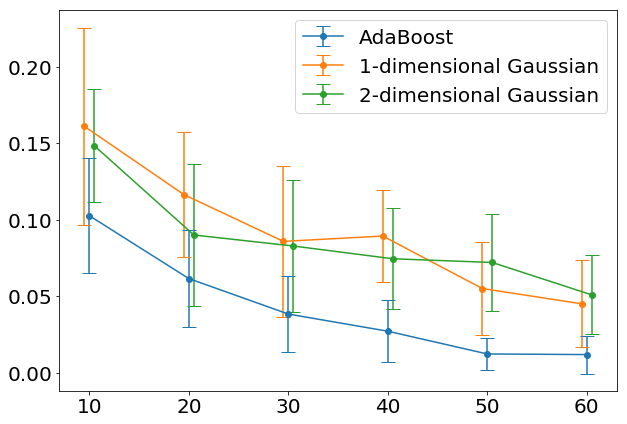
\includegraphics[width=8cm, height=5cm]{Figures/Mushroom_labelProp_vs_AdaBoost.png}
%     \caption{Comparing Label Propagation with AdaBoost on the Mushroom Dataset.}
%     \label{fig:lp_vs_AdaBoost_mushroom}
% \end{figure}

% \noindent{\textbf{Congressional Voting Record:}}
% The Congressional Voting Record dataset from UCI machine learning repository comprises the voting record the $2$nd session of the $98$th Congress  on $16$ issues. We form $2$ hyperedges for each issue, and hence $32$ in total, with one containing voters who voted ``Yay'' and the other, ``Nay''. There were voters whose votes were missing, but we do not assign hyperedges for them. We point out yet another desirable property of label propagation made clear by this example that we don't have find a way to treat missing values, as required by most classification algorithms -- since the votes were missing for miscellaneous reasons, there may not be a uniformly sensible way of assignment. We test label propagation algorithm with $5$, $10$, $15$, $20$, $25$, and $30$ congressmen and women from each party whose affiliation are given, and we benchmark our results with those of AdaBoost. See Fig.~\ref{fig:lp_vs_AdaBoost_congress}.
% \begin{figure}[ht]
%     \centering
%     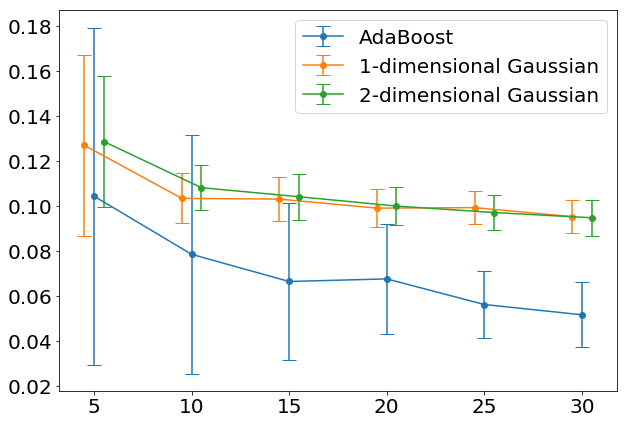
\includegraphics[width=8cm, height=5cm]{Figures/Congress_labelProp_vs_AdaBoost.png}
%     \caption{Comparing Label Propagation with AdaBoost on the Congress Dataset.}
%     \label{fig:lp_vs_AdaBoost_congress}
% \end{figure}

% \subsection{Web of Science 2015 AI Papers}
% The WoS AI paper dataset comprise $1573$ authors and $12948$ papers in Artificial Intelligence published in year 2015. They hypergraph is formed with hyperedges being authors, vertices being papers, and incidency defined by authorship. We first do a topic modelling on the abstracts with $5$ topics, and use the clusters obtained from running spectral clustering on the topic distributions as ground truth. Then, for each topic, we pick $20$ papers with topic distribution the most concentrated on that topic as labeled data, and propagate the known topic distributions through the network. To show the performance of label propagation, we compare the clusters obtained with running spectral clustering on propagated distributions with those calculated directly from topic modelling.

\section{Conclusion}
In this paper, we proposed a novel framework for a semi-supervised learning problem where (i) the labels are given by probability measures on a metric space (aka soft labels) and (ii) the underlying similarity structure is given by a hypergraph (which subsumes graph and simplicial complex). Our framework was inspired by a re-formulation of graph-based label propagation in terms of message passing and borrowed ideas from the theory of multi-marginal optimal transport. We then established generalization error bounds for propagating one-dimensional distributions using $2$-Wasserstein distances. To the best of our knowledge, this constitutes the first generalization error bounds for Wasserstein distance based soft label propagation, even on graphs. We expect similar generalization bounds to hold for propagating higher-dimensional probability distributions as well as using other Wasserstein distances, but a deeper understanding of the geometry of Wasserstein spaces will be indispensable for those purposes.
	
	
\bibliography{bibliography}
\bibliographystyle{aaai}	




	\clearpage
	\section{Appendix}
	
	

		Below are the supplemental material for the paper  "Wasserstein Soft Label Propagation on Hypergraphs: Algorithm and Generalization Error Bounds"   submitted to AAAI 2019 

	
	\subsection{Proof of Lemma~\ref{lem:maximum-principle}}
	The conditions on $\Phi$ can be written as
	\begin{align}
	\left[\frac{t_i}{m\gamma}+\mathrm{deg}\left(i\right)\right]\Phi \left( i \right)-\sum_{j:j\sim i}\Phi \left( j \right)\geq 0 & \qquad 1\leq i\leq \ell\label{eq:maximum-principle-boundary}\\
	\mathrm{deg}\left(i\right)\Phi \left( i \right)-\sum_{j:j\sim i}\Phi \left( j \right)=0 & \qquad \ell+1\leq i\leq n\label{eq:maximum-principle-interior}
	\end{align}
	where $\mathrm{deg}\left( i \right)\geq 1$ is the degree of vertex $i$ in graph $G$. First, we assert that the minimum of $\Phi$ must be attained among the vertices $1,\cdots,\ell$, for otherwise, if $\ell+1\leq i_*=\argmin_{i\in V}\Phi \left( i \right)\leq n$, then by \eqref{eq:maximum-principle-interior} we have
	\begin{equation*}
	\begin{aligned}
	\mathrm{deg}\left(i_*\right)\Phi \left( i_* \right)&=\sum_{j:j\sim i_*}\Phi \left( j \right)\\
	&\geq \sum_{j:j\sim i_*}\Phi \left( i_* \right)=\mathrm{deg}\left(i_*\right)\Phi \left( i_* \right)
	\end{aligned}
	\end{equation*}
	which implies $\Phi \left( j \right)=\Phi \left( i_* \right)$ for all vertices $j\sim i_*$. This argument can be repeated until the constant value propagates into the vertices within $1,\cdots,\ell$, and the assertion follows from the connectivity of the graph. The assertion for the maximum can be established analogously. Next we argue that the minimum of $\Phi$ on the vertices of $G$ must be non-negative. Assume the contracy, i.e. the minimum attained at $i_*\in \left[ 1,\ell \right]$ is strictly negative, then by \eqref{eq:maximum-principle-boundary} we have
	\begin{equation*}
	\begin{aligned}
	0 &\leq \left[\frac{t_{i_*}}{m\gamma}+\mathrm{deg}\left(i_{*}\right)\right]\Phi \left( i_{*} \right)-\sum_{j:j\sim i_{*}}\Phi \left( j \right)\\
	&=\frac{t_{i_*}}{m\gamma}\Phi \left( i_* \right)+\sum_{j:j\sim i_*}\left[ \Phi \left( i_* \right)-\Phi \left( j \right) \right]<0
	\end{aligned}
	\end{equation*}
	where the strict inequalty follows from the counter-assumption $\Phi \left( i_{*} \right)<0$. This contradiction completes our proof that $\Phi \geq 0$ on the entire graph $G$.
	
% 	\subsection{Proof of Proposition~\ref{Propo:Non_Decreasing}}
% 	By the equivalence of \eqref{eq:tikhonov-one-dimensional-subproblem-equiv} and \eqref{eq:tikhonov-one-dimensional-subproblem}, the solutions $\Phi_s$ satisfies the Euler-Lagrange equations for \eqref{eq:tikhonov-one-dimensional-subproblem}:
% 	\begin{equation*}
% 	\left( T_{\ell}+m\gamma L \right)\Phi_s^{*}=\mathbf{y}_s.
% 	\end{equation*}
% 	For any $0\leq t\leq s\leq 1$, subtracting two Euler-Lagrange equations yields
% 	\begin{equation*}
% 	\left( T_{\ell}+m\gamma L \right)\left(\Phi_s^{*}-\Phi_t^{*}\right)=\mathbf{y}_s-\mathbf{y}_t\geq 0
% 	\end{equation*}
% 	where the inequality follows from the definition of $\mathbf{y}_s$ in \eqref{eq:y-defn}. Furthermore, it is straightforward to see that $\mathbf{y}_s-\mathbf{y}_t$ satisfies the assumption in Lemma~\ref{lem:maximum-principle}, which then implies $\Phi_s^{*}\geq \Phi_t^{*}$.
	
	\subsection{Proof of Theorem~\ref{thm:slice-algorithmic-stability}}
	Following the same argument as in the proof of \cite[Theorem 5]{Belkin2004}, we can assume without loss of generality that $S$, $S'$ differ by a new point $\left( v_m,\mu_m \right)\leftrightarrow \left( v_m',\mu_m' \right)$; the other case where only the multiplicities differ can be treated similarly. By our assumption \eqref{eq:quantile-boundedness}, the two averages differ by at most an amount of
	\begin{equation*}
	\left| \bar{y}_s-\bar{y}_s' \right|\leq \frac{2M_s}{m}.
	\end{equation*}
	For simplicity, introduce temporary notations
	\begin{equation*}
	A:=T_{\ell}+m\gamma L,\qquad B:=T_{\ell}'+m\gamma L.
	\end{equation*}
	Using the simple fact that the $2$-norm dominate the $\infty$-norm, we have
	\begin{equation*}
	\begin{aligned}
	&\left\| \Phi_s^{*} -\Phi_s'^{*} \right\|_{\infty} \leq \left\| \Phi_s^{*} -\Phi_s'^{*} \right\|_2\\
	&\leq \frac{2M_s}{m}+\left\| A^{-1}\left(\mathbf{y}_s-\bar{y}_sT_\ell\mathbf{1}\right)-B^{-1}\left(\mathbf{y'}_s-\bar{y}_s'T'_\ell\mathbf{1}\right) \right\|_2\\
	&\leq \frac{2M_s}{m}+\left\| A^{-1}\left(\mathbf{y}_s-\bar{y}_sT_\ell\mathbf{1}\right)-A^{-1}\left(\mathbf{y'}_s-\bar{y}_s'T'_\ell\mathbf{1}\right) \right\|_2\\
	&\qquad+\left\| A^{-1}\left(\mathbf{y'}_s-\bar{y}_s'T'_\ell\mathbf{1}\right)-B^{-1}\left(\mathbf{y'}_s-\bar{y}_s'T'_\ell\mathbf{1}\right) \right\|_2.
	\end{aligned}
	\end{equation*}
	Stanard functional analysis argument (the same perturbation reasoning we gave in \eqref{eq:standard-functional-analysis}) tells us that $\left\| A^{-1} \right\|_2\leq \left( m\gamma\lambda_1-T \right)^{-1}$. Together with the observation that
	\begin{align*}
	&\left\| \left(\mathbf{y}_s-\bar{y}_sT_\ell\mathbf{1}\right) - \left(\mathbf{y'}_s-\bar{y}_s'T'_\ell\mathbf{1}\right) \right\|_2\\
	&\leq \left\| \mathbf{y}_s-\mathbf{y}_s' \right\|_2+\left\| \bar{y}_sT_\ell\mathbf{1}-\bar{y}_s'T'_\ell\mathbf{1} \right\|_2\\
	&\leq 2M_s+\frac{2M_s}{m}<4M_s
	\end{align*}
	we have
	\begin{equation*}
	\left\| A^{-1}\left(\mathbf{y}_s-\bar{y}_sT_\ell\mathbf{1}\right)-A^{-1}\left(\mathbf{y'}_s-\bar{y}_s'T'_\ell\mathbf{1}\right) \right\|_2\leq \frac{4M_s}{m\gamma\lambda_1-T}.
	\end{equation*}
	In the meanwhile, noting that we also have $\left\| B^{-1} \right\|_2\leq \left( m\gamma\lambda_1-T \right)^{-1}$, and $\left\| A-B \right\|_2=\left\| T_{\ell}'-T_{\ell} \right\|_2 \leq \sqrt{2}<3/2$, we conclude that
	\begin{equation*}
	\begin{aligned}
	&\left\| A^{-1}\left(\mathbf{y'}_s-\bar{y}_s'T'_\ell\mathbf{1}\right)-B^{-1}\left(\mathbf{y'}_s-\bar{y}_s'T'_\ell\mathbf{1}\right) \right\|_2\\
	&=\left\| B^{-1} \left( B-A \right) A^{-1}\left(\mathbf{y'}_s-\bar{y}_s'T'_\ell\mathbf{1}\right)\right\|_2\leq \frac{3M_s\sqrt{Tm}}{\left( m\gamma\lambda_1-T \right)^2}.
	\end{aligned}
	\end{equation*}
	Putting everything together completes the proof.
	
% 	\subsection{Proof of Lemma~\ref{lem:apriori-estimates}}
	
% 	By the equivalence between \eqref{eq:tikhonov} and \eqref{eq:tikhonov-one-dimensional}, it suffices to show the following fact: for each fixed $s\in \left[ 0,1 \right]$, if $\max \left\{ \left|F_{\mu_i}^{-1} \left( s \right)\right|,\,\,i=1,\cdots,m\right\}\leq \phi \left( s \right)$ then $\left\|\Phi_s^{*}\right\|_{\infty}\leq \phi \left( s \right)$, where $\Phi_s^{*}$ is defined in \eqref{eq:tikhonov-one-dimensional-subproblem-equiv}. But this follows straightforwardly from the maximum principle.
	
	
% % 	\subsection{Proof of Proposition~\ref{prop:alg-stability-slp}}
% % 	Let $\left( j,\theta_j \right)$ be a new sample drawn from the joint distribution $D$. Then $\theta_j\in\mathcal{M}_{\phi}^2$ with probability $1$. Let $S$, $S'$ be two training samples with values in $\mathcal{M}_{\phi}^2$ and differ by exactly one data point. By Theorem~\ref{thm:slice-algorithmic-stability} we have
% % 	\begin{equation}
% % 	\label{eq:sliced-bounds}
% % 	\begin{aligned}
% % 	&\left| \Phi_s^{*} \left( j \right) -\Phi_s'^{*} \left( j \right) \right| \\
% % 	&\leq \left[\frac{3\sqrt{Tm}}{\left( m\gamma\lambda_1-T \right)^2}+\frac{4}{m\gamma\lambda_1-T}+\frac{2}{m}\right]\phi \left( s \right).
% % 	\end{aligned}
% % 	\end{equation}
% % 	%  By \eqref{eq:one-dimensional-wasserstein},
% % 	By \eqref{Eq:One_D_Equivalence}, the difference between the squared Wasserstein losses satisfy
% % 	\begin{equation*}
% % 	\begin{aligned}
% % 	&\left| c \left( f_S, \left( j,\theta_j \right) \right) - c \left( f_{S'}, \left( j,\theta_j \right) \right) \right|\\
% % 	&=\left| W_2^2 \left( f_S \left( j \right),\theta_j \right) - W_2^2 \left( f_{S'} \left( j \right),\theta_j \right) \right|\\
% % 	&=\left| \int_0^1 \left| \Phi_s^{*} \left( j \right)-F_{\theta_j}^{-1}\left( s \right) \right|^2\mathrm{d}s - \int_0^1 \left| \Phi_s'^{*} \left( j \right)-F_{\theta_j}^{-1}\left( s \right) \right|^2\mathrm{d}s \right|\\
% % 	&\leq \int_0^1 \left| \left( \Phi_s^{*} \left( j \right)+\Phi_s'^{*} \left( j \right)-2F_{\theta_j}^{-1}\left( s \right) \right)\left( \Phi_s^{*} \left( j \right) -\Phi_s'^{*} \left( j \right) \right) \right| \mathrm{d}s\\
% % 	&\stackrel{\left( * \right)}{\leq} \left[\frac{3\sqrt{Tm}}{\left( m\gamma\lambda_1-T \right)^2}+\frac{4}{m\gamma\lambda_1-T}+\frac{2}{m}\right]\cdot \int_0^1 4\phi \left( s \right)\cdot \phi \left( s \right)\mathrm{d}s\\
% % 	&=4\left\| \phi \right\|_2^2\left[\frac{3\sqrt{Tm}}{\left( m\gamma\lambda_1-T \right)^2}+\frac{4}{m\gamma\lambda_1-T}+\frac{2}{m}\right]=\beta,
% % 	\end{aligned}
% % 	\end{equation*}
% % 	where at $\left( * \right)$ we used \eqref{eq:sliced-bounds} to bound the difference $\left| \Phi_s^{*} \left( j \right) -\Phi_s'^{*} \left( j \right) \right|$, and invoked Lemma~\ref{lem:apriori-estimates} to conclude that
% % 	\begin{equation*}
% % 	\Phi_s^{*}\left( j \right),\Phi_s'^{*}\left( j \right) \leq \phi \left( s \right)
% % 	\end{equation*}
% % 	and hence
% % 	\begin{equation*}
% % 	\left| \Phi_s^{*} \left( j \right)+\Phi_s'^{*} \left( j \right)-2F_{\theta_j}^{-1}\left( s \right) \right|\leq 4\phi \left( s \right).
% % 	\end{equation*}
	
	
% % 	\subsection{Proof of Theorem~\ref{Thm:Gen_Error_Soft}}
	
	
% % 	Note that the cost function is uniformly bounded by $M=4 \left\| \phi \right\|_2^2$ in our setting. The rest follows from Proposition~\ref{prop:alg-stability-slp} and Theorem~\ref{thm:bousquet-elisseeff}.
	
	
	
	
	
	
	



\end{document}

